%%%%%%%%%%%%%%%%%%%%%%%%%%%%%%%%%%%%%%%%%%%%%%%%
%% Compile the master file!
%% 		Slides: Antonio Machicao y Priemer
%% 		Course: GK Linguistik
%%%%%%%%%%%%%%%%%%%%%%%%%%%%%%%%%%%%%%%%%%%%%%%%


%%%%%%%%%%%%%%%%%%%%%%%%%%%%%%%%%%%%%%%%%%%%%%%%%%%%
%%%             Metadata                         
%%%%%%%%%%%%%%%%%%%%%%%%%%%%%%%%%%%%%%%%%%%%%%%%%%%%      

\title{Grundkurs Linguistik}

\subtitle{Syntax VI: X-Bar-Theorie -- Funktionale Phrasen}

\author[aMyP]{
	{\small Antonio Machicao y Priemer}
	\\
	{\footnotesize \url{http://www.linguistik.hu-berlin.de/staff/amyp}}
%	\\
%	{\footnotesize \href{mailto:mapriema@hu-berlin.de}{mapriema@hu-berlin.de}}
}

\institute{Institut für deutsche Sprache und Linguistik}

\date{ }

%\publishers{\textbf{6. linguistischer Methodenworkshop \\ Humboldt-Universität zu Berlin}}

%\hyphenation{nobreak}


%%%%%%%%%%%%%%%%%%%%%%%%%%%%%%%%%%%%%%%%%%%%%%%%%%%%
%%%             Preamble's End                   %%%
%%%%%%%%%%%%%%%%%%%%%%%%%%%%%%%%%%%%%%%%%%%%%%%%%%%%      


%%%%%%%%%%%%%%%%%%%%%%%%%      
\huberlintitlepage
\iftoggle{toc}{
\frame{
\begin{multicols}{2}
	\frametitle{Inhaltsverzeichnis}\tableofcontents
	%[pausesections]
\end{multicols}
	}
	}


%%%%%%%%%%%%%%%%%%%%%%%%%%%%%%%%%%
%%%%%%%%%%%%%%%%%%%%%%%%%%%%%%%%%%
%%%%%LITERATURE:

%\nocite{Altmann&Hofmann08a}
%\nocite{Altmann93a}
\nocite{Brandt&Co06a}
\nocite{Glueck05a} 
\nocite{Grewendorf&Co91a} 
\nocite{Luedeling2009a} 
%\nocite{Meibauer&Co07a}
\nocite{MuellerS13f} 
\nocite{MuellerS15b}
%% Allgemein
\nocite{Glueck&Roedel16a}
%\nocite{Meibauer&Co07a} 
\nocite{Repp&Co15a} 

%% Morphologie
%\nocite{Eisenberg04}

%% Syntax
\nocite{Adger04a}
%\nocite{Altmann&Hofmann08a} % Satztypen & Satzmodi
%\nocite{Altmann93a} % Satztypen & Satzmodi
\nocite{Brandt&Co06a} 
\nocite{Fanselow&Sascha87a}
\nocite{Fanselow&Sascha93a}
%\nocite{Fries&MyP16b} % Akzeptabilität
%\nocite{Fries16a} % Grammatikalität
%\nocite{Fries&MyP16d} % Kompetenz vs Performanz
\nocite{Fries&MyP16c} % GG
\nocite{Fries&MyP16a} % X-Bar-Theorie
%\nocite{Fries16e} % Satztyp
%\nocite{Fries16d} % Satzmodus 
\nocite{Grewendorf&Co91a} 
%\nocite{MyP17b} % Kerngrammatik
%\nocite{MyP18a} % Konstituententest
\nocite{MyP18b} % Kopf
\nocite{MyP18c} % Phrase
\nocite{MyP18s} % Funktionale Kategorie
\nocite{MyP18t} % Argumentstruktur
%\nocite{MuellerS13f} 
%\nocite{MuellerS15b}
\nocite{Stechow&Sternefeld88a}
\nocite{Sternefeld06a}
\nocite{Sternefeld06b}
%\nocite{Woellstein10a} % Topologisches Feldermodell


%%%%%%%%%%%%%%%%%%%%%%%%%%%%%%%%%
\section{Syntax VI}
%%%%%%%%%%%%%%%%%%%%%%%%%%%%%%%%%

\subsection{Begriffe: GG vs. Traditionell}

\iftoggle{sectoc}{
	\frame{
		%\begin{multicols}{2}
		\frametitle{~}
		\tableofcontents[currentsubsection,subsubsectionstyle=hide]
		%\end{multicols}
	}
}


%%%%%%%%%%%%%%%%%%%%%%%%%%%%%%%%%%%
\begin{frame}
\frametitle{Begriffe: GG \vs Traditionell}

\begin{itemize}
	\item Die Begriffe in der \textbf{traditionellen Grammatik} (UE) und in anderen syntaktischen Theorien (Valenz, \textbf{GG}, \dots ) sind nicht vollkommen gleichzusetzen, weil sie auch nicht die gleichen \textbf{Kategorien} bezeichnen!
	\item[]
	\item Es gibt Bereiche, in denen die Begriffe Ähnliches bezeichnen, aber \idR  haben sie verschiedene Reichweiten.
	\item[]
	\item Kurze Gegenüberstellung zur begrifflichen Klärung \dots
	\item[]
	\item $\approx$ \ras ungefähr
\end{itemize}

\end{frame}


%%%%%%%%%%%%%%%%%%%%%%%%%%%%%%%%%%
\begin{frame}
\frametitle{Begriffe: GG \vs Traditionell}

\begin{minipage}[b]{0.47\textwidth}

	\textbf{GG:}

	\begin{itemize}
		\item \alertred{\textbf{Argumente:}}
		\begin{itemize}
			\item (aus der Semantik entlehnter Begriff)
			
			\item Leerstellen einer Kategorie \zerobar{X}
			
			\item \textbf{Externes Argument + Komplemente}
		\end{itemize}

		\item[]

		\item \textbf{Komplemente:}
		\begin{itemize}
			\item interne Argumente
		\end{itemize}

	\end{itemize}	
\end{minipage}  
  	  %
  	  %
\begin{minipage}[b]{0.5\textwidth}
	\begin{figure}
	\centering
	\scalebox{.55}{
		\begin{forest}
		sm edges,
		[?P [DP [Die Dame,roof]],tikz={\node [draw,red,fit=()] {};} 
			[\MyPxbar{?} 		
		[VP [AdvP [schnell,roof]]
			[VP [DP [dem Jungen,roof]],tikz={\node [draw,red,fit=()] {};}
		    [\MyPxbar{V}	[DP [den Wagen,roof]],tikz={\node [draw,red,fit=()] {};}				
		    			[\zerobar{V} [schenken]]
			]]
		]
			[\zerobar{?} [~]]
		]]			 
		\end{forest}
		}         
	\end{figure}
\end{minipage}

\end{frame}


%%%%%%%%%%%%%%%%%%%%%%%%%%%%%%%%%%
\begin{frame}
\frametitle{Begriffe: GG \vs Traditionell}

\begin{minipage}[b]{0.47\textwidth}

	\textbf{GG:}

	\begin{itemize}
		\item \textbf{Argumente:}
		\begin{itemize}
			\item (aus der Semantik entlehnter Begriff)
			
			\item Leerstellen einer Kategorie \zerobar{X}
			
			\item \textbf{Externes Argument + Komplemente}
		\end{itemize}
		
		\item[]
		
		\item \alertred{\textbf{Komplemente:}}
		\begin{itemize}
			\item interne Argumente
		\end{itemize}
		
	\end{itemize}	
\end{minipage}  
  	%  
  	%  
\begin{minipage}[b]{0.48\textwidth}
	\begin{figure}
	\centering
	\scalebox{.55}{
		\begin{forest}
		sm edges,
		[?P [DP [Die Dame,roof]]
			[\MyPxbar{?} 		
		[VP [AdvP [schnell,roof]]
			[\alertred{VP} [DP [dem Jungen,roof]],tikz={\node [draw,red,fit=()] {};}
		    [\MyPxbar{V}	[DP [den Wagen,roof]],tikz={\node [draw,red,fit=()] {};}				
		    			[\zerobar{V} [schenken]]
			]]
		]
			[\zerobar{?} [~]]
		]]			 
		\end{forest}
		}

	\end{figure}
\end{minipage}

\end{frame}


%%%%%%%%%%%%%%%%%%%%%%%%%%%%%%%%%%
\begin{frame}
\frametitle{Begriffe: GG \vs Traditionell}

\begin{minipage}[b]{0.47\textwidth}

	\textbf{GG:}

	\begin{itemize}
		\item \alertred{\textbf{Externes Argument:}}\\
		Argument von \zerobar{X}, dessen Basisposition \textbf{außerhalb} der XP liegt
		\item[]
		\item \textbf{Internes Argument:}\\
		Argument von \zerobar{X}, dessen Basisposition \textbf{innerhalb} der XP liegt
	\end{itemize}	
\end{minipage}  
  	%  
  	%  
\begin{minipage}[b]{0.48\textwidth}
	\begin{figure}
	\centering
	\scalebox{.55}{
		\begin{forest}
		sm edges,
		[\alertred{?P} [DP [Die Dame,roof]],tikz={\node [draw,red,fit=()] {};}
			[\MyPxbar{?} 		
		[VP [AdvP [schnell,roof]]
			[\alert{VP} [DP [dem Jungen,roof]]
		    [\MyPxbar{V}	[DP [den Wagen,roof]]
		    			[\zerobar{V} [schenken]]
			]]
		]
			[\zerobar{?} [~]]
		]]			 
		\end{forest}
		}
	\end{figure}
\end{minipage}    

\end{frame}


%%%%%%%%%%%%%%%%%%%%%%%%%%%%%%%%%%
\begin{frame}
\frametitle{Begriffe: GG \vs Traditionell}

\begin{minipage}[b]{0.47\textwidth}

	\textbf{GG:}
	\begin{itemize}
		\item \textbf{Externes Argument:}\\
		Argument von \zerobar{X}, dessen Basisposition \textbf{außerhalb} der XP liegt
		\item[]
		\item \textbf{Internes Argument:}\\
		Argument von \zerobar{X}, dessen Basisposition \textbf{innerhalb} der XP liegt
	\end{itemize}	
\end{minipage}  
  	%  
  	%  
\begin{minipage}[b]{0.48\textwidth}
	\begin{figure}
	\centering
	\scalebox{.55}{
		\begin{forest}
		sm edges,
		[?P [DP [Die Dame,roof]]
			[\MyPxbar{?} 		
		[VP [AdvP [schnell,roof]]
			[\alertred{VP} [DP [dem Jungen,roof]],tikz={\node [draw,red,fit=()] {};}
		    [\MyPxbar{V}	[DP [den Wagen,roof]],tikz={\node [draw,red,fit=()] {};}
		    			[\zerobar{V} [schenken]]
			]]
		]
			[\zerobar{?} [~]]
		]]			 
		\end{forest}
		}
	\end{figure}	
\end{minipage}

\end{frame}


%%%%%%%%%%%%%%%%%%%%%%%%%%%%%%%%%%
\begin{frame}
\frametitle{Begriffe: GG \vs Traditionell}

\begin{minipage}[b]{0.4\textwidth}

	\textbf{Traditionell (UE):}
		\begin{itemize}
		\item \alertred{\textbf{Subjekt}}\\
		$\approx$ Externes Argument in GG
		\item[]
		\item \textbf{Objekte}\\
		$\approx$ Komplemente oder interne Argumente in GG
		\end{itemize}	
\end{minipage}  
  	%  
  	%  
\begin{minipage}[b]{0.55\textwidth}
	\begin{figure}
	\centering
	\scalebox{.6}{
		\begin{forest}
		sm edges,
		[\alertred{?P} [DP [Die Dame,roof]],tikz={\node [draw,red,fit=()] {};}
			[\MyPxbar{?} 		
		[VP [AdvP [schnell,roof]]
			[\alert{VP} [DP [dem Jungen,roof]]
		    [\MyPxbar{V}	[DP [den Wagen,roof]]
		    			[\zerobar{V} [schenken]]
			]]
		]
			[\zerobar{?} [~]]
		]]			 
		\end{forest}
		}
	\end{figure}	
\end{minipage}

\end{frame}


%%%%%%%%%%%%%%%%%%%%%%%%%%%%%%%%%%
\begin{frame}
\frametitle{Begriffe: GG \vs Traditionell}

\begin{minipage}[b]{0.4\textwidth}
	\footnotesize
	\textbf{Traditionell (UE):}
		\begin{itemize}
		\item \textbf{Subjekt}\\
		$\approx$ Externes Argument in GG
		\item[]
		\item \alertred{\textbf{Objekte}}\\
		$\approx$ Komplemente oder interne Argumente in GG
		\end{itemize}	
  	\end{minipage}  
  	%  
  	%  
	\begin{minipage}[b]{0.55\textwidth}
		\begin{figure}
	\centering
	\scalebox{.6}{
		\begin{forest}
		sm edges,
		[?P [DP [Die Dame,roof]]
			[\MyPxbar{?} 		
		[VP [AdvP [schnell,roof]]
			[\alertred{VP} [DP [dem Jungen,roof]],tikz={\node [draw,red,fit=()] {};}
		    [\MyPxbar{V}	[DP [den Wagen,roof]],tikz={\node [draw,red,fit=()] {};}
		    			[\zerobar{V} [schenken]]
			]]
		]
			[\zerobar{?} [~]]
		]]			 
		\end{forest}
		}
	
	\end{figure}
\end{minipage}

\end{frame}


%%%%%%%%%%%%%%%%%%%%%%%%%%%%%%%%%%
\begin{frame}
\frametitle{Begriffe: GG \vs Traditionell}

\begin{minipage}[b]{0.49\textwidth}
	\textbf{ABER!!}	\\
	\textbf{GG vs. Traditionell}
		\begin{itemize}
		\item \textbf{Externes Argument}\\
		$\neq$ Subjekt (in trad. Terminologie)
		\item<2>[\ra] \alertred{\textbf{Genitivattribut}}
		\item[]
		\item \textbf{Komplement}\\
		$\neq$ Objekt (in trad. Terminologie)
		\item<2>[\ra] \alertred{\textbf{Genitivattribut}}
		\item[]
		\end{itemize}	
  	\end{minipage}  
  	%  
	\begin{minipage}[b]{0.46\textwidth}
	\centering
	\footnotesize{
		\begin{forest}
		MyP edges,
		[?P
		[DP [Peters,roof]]	,tikz={\node [draw,red,fit=()] {};}	
		[\MyPxbar{?} [\zerobar{?}]
			[\alertred{NP} 
		    [\MyPxbar{N}	[\zerobar{N} [Behandlung]]
					 	[DP [des Patienten,roof]],tikz={\node [draw,red,fit=()] {};}
			]]
		]
		]			 
		\end{forest}
		}

\end{minipage}

\end{frame}


%%%%%%%%%%%%%%%%%%%%%%%%%%%%%%%%%%
\begin{frame}
\frametitle{Begriffe: GG \vs Traditionell}

\begin{minipage}[b]{0.49\textwidth}
	\textbf{ABER!!}	\\
	\textbf{GG vs. Traditionell}
		\begin{itemize}
		\item \textbf{Traditionell:} Die Begriffe \gqq{Subjekt} und \gqq{Objekt} sind \textbf{nur für Satzglieder} definiert, nicht für Satzgliedteile (Attribute).
		\item[]
		\item \textbf{GG:} Die Begriffe \gqq{Argument} und \gqq{Komplement} sind für \textbf{Relationen zwischen Phrasen} in allen Phrasentypen definiert.
		\end{itemize}	
  	\end{minipage}  
  	%  
	\begin{minipage}[b]{0.46\textwidth}
	\centering
	\footnotesize{
		\begin{forest}
		MyP edges,
		[?P
		[DP [Peters,roof]]	,tikz={\node [draw,red,fit=()] {};}	
		[\MyPxbar{?} [\zerobar{?}]
			[\alertred{NP} 
		    [\MyPxbar{N}	[\zerobar{N} [Behandlung]]
					 	[DP [des Patienten,roof]],tikz={\node [draw,red,fit=()] {};}
			]]
		]
		]			 
		\end{forest}
		}
\end{minipage}

\end{frame}


%%%%%%%%%%%%%%%%%%%%%%%%%%%%%%%%%%
\begin{frame}
\frametitle{Begriffe: GG \vs Traditionell}

\begin{minipage}[b]{0.45\textwidth}
%	\footnotesize
	\textbf{GG:}
		\begin{itemize}
		\item \textbf{Modifikator}
		
		\begin{itemize}
			\item (aus der Semantik entlehnter Begriff)
			
			\item Synt. Begriff: \textbf{Adjunkt}
		\end{itemize}

%		\item[]

		\item Adjunkte werden \textbf{traditionell}\\
		\alertred{\textbf{Adverbiale}} (Adjunkte, die Satzglieder sind)\\
		oder\\
		\textbf{Attribute} (Adjunkte, die Satzgliedteile sind)\\
		genannt.
		\end{itemize}	
  	\end{minipage}  
  	%  
  	%  
\begin{minipage}[b]{0.5\textwidth}
	\centering
	\scalebox{.55}{
		\begin{forest}
		sm edges,
		[?P [DP [Die Dame,roof]]
			[\MyPxbar{?} 		
		[VP [AdvP [schnell,roof]],tikz={\node [draw,red,fit=()] {};}
			[\alert{VP} [DP [dem Jungen,roof]]
		    [\MyPxbar{V}	[DP [den Wagen,roof]]
		    			[\zerobar{V} [schenken]]
			]]
		]
			[\zerobar{?} [~]]
		]]			 
		\end{forest}
		}
\end{minipage}
  
\end{frame}


%%%%%%%%%%%%%%%%%%%%%%%%%%%%%%%%%%
\begin{frame}
\frametitle{Begriffe: GG \vs Traditionell}

\begin{minipage}[b]{0.45\textwidth}
%	\footnotesize
	\textbf{GG:}
		\begin{itemize}
		\item \textbf{Modifikator}\\
		(aus der Semantik entlehnter Begriff)\\
		Syntaktischer Begriff: \textbf{Adjunkt}
		\item[]
		\item Adjunkte werden \textbf{traditionell}\\
		\textbf{Adverbiale}	(Adjunkte, die Satzglieder sind)\\
		oder\\
		\alertred{\textbf{Attribute}} (Adjunkte, die Satzgliedteile sind)\\
		genannt.
		\end{itemize}	
\end{minipage}  
  	%  
  	%  
\begin{minipage}[b]{0.5\textwidth}
	\begin{figure}
	\centering
	\scalebox{.65}{
		\begin{forest}
		MyP edges,
		[?P
		[DP [Peters,roof]]	
		[\MyPxbar{?} [\zerobar{?}]
			[NP [AP [schnelle,roof]],tikz={\node [draw,red,fit=()] {};}	 
			[\alertred{NP} 
		    [\MyPxbar{N}	[\zerobar{N} [Behandlung]]
					 	[DP [des Patienten,roof]]
			]]]
		]
		]			 
		\end{forest}
		}

	\end{figure}	
\end{minipage}

\end{frame}


%%%%%%%%%%%%%%%%%%%%%%%%%%%%%%%%%
%%%%%%%%%%%%%%%%%%%%%%%%%%%%%%%%%
\subsection{Weiteres zum X-Bar-Schema}

\iftoggle{sectoc}{
	\frame{
		%\begin{multicols}{2}
		\frametitle{~}
		\tableofcontents[currentsubsection,subsubsectionstyle=hide]
		%\end{multicols}
	}
}


%%%%%%%%%%%%%%%%%%%%%%%%%%%%%%%%%%%%
\begin{frame}
\frametitle{Weiteres zum X-Bar-Schema}


\begin{minipage}[b]{0.45\textwidth}
	\begin{itemize}
		\item \textbf{Mutter}
		\item \textbf{Tochter}
		\item Schwester
	\end{itemize}
\end{minipage}  
%
%
	\begin{minipage}[b]{0.45\textwidth}
	\centering
	\footnotesize{
		\begin{forest}
		MyP edges,
		[\alert{XP} [\alert{YP}]{\draw[<-,red] (.north west)--++(0em,+3ex)--++(-2.5em,0pt)
node[anchor=east,align=center]{Tochter};}
			[\alert{\MyPxbar{X}}
				[\zerobar{X}]
				[ZP]
			]{\draw[<-,red] (.north east)--++(-0em,+2ex)--++(+2.5em,0pt)
node[anchor=west,align=center]{Tochter};} 
		]{\draw[<-,red] (.north east)--++(-0em,+2ex)--++(+2.5em,0pt)
node[anchor=west,align=center]{Mutter};} 
		\end{forest}
		}

\end{minipage}  

\end{frame}


%%%%%%%%%%%%%%%%%%%%%%%%%%%%%%%%%%%%
\begin{frame}
\frametitle{Weiteres zum X-Bar-Schema}


\begin{minipage}[b]{0.45\textwidth}
	\begin{itemize}
		\item Mutter
		\item Tochter
		\item \textbf{Schwester}
		\item[]
		\item Präferierte Position für \textbf{Komplemente} \ras Schwesterkonstituente des Kopfes (s.\ ZP)
		
	\end{itemize}
\end{minipage}  
%
% 
\begin{minipage}[b]{0.5\textwidth}
	\centering
	\footnotesize{
		\begin{forest}
		MyP edges,
		[XP [\alert{YP}]{\draw[<-,red] (.north west)--++(0em,+3ex)--++(-2.5em,0pt)
node[anchor=east,align=center]{Schwester};}
			[\alert{\MyPxbar{X}}
				[\zerobar{X}]
				[ZP]
			]{\draw[<-,red] (.north east)--++(-0em,+2ex)--++(+2.5em,0pt)
node[anchor=west,align=center]{Schwester};} 
		]
		\end{forest}
		}
\end{minipage}  

\nocite{MyP17d}

\end{frame}


%%%%%%%%%%%%%%%%%%%%%%%%%%%%%%%%%%%%
\begin{frame}
\frametitle{Weiteres zum X-Bar-Schema}

\begin{itemize}
	\item Die \textbf{Position des Kopfes} (rechts oder links) ist sprach- und phrasenabhängig,
	\begin{itemize}
		\item VP im Deutschen \ras \alertred{rechts}köpfig
		\item VP im Englischen \ras \alertred{links}köpfig			
	\end{itemize}
\end{itemize}
	
\begin{minipage}[b]{0.45\textwidth}
\begin{figure}	
	\centering
	\footnotesize{
		\begin{forest}
		sm edges,
		[VP	[\MyPxbar{V}
					[\alertred{\zerobar{V}} [(to) buy]]
					[DP [a car,roof]]
			]
		]
		\end{forest}
		}
		\caption{VP Englisch}
\end{figure}	
\end{minipage}  
%
%           
\begin{minipage}[b]{0.45\textwidth}
\begin{figure}
	\centering
	\footnotesize{
		\begin{forest}
		sm edges,
		[VP	[\MyPxbar{V}
					[DP [einen Wagen,roof]]
					[\alertred{\zerobar{V}} [(zu) kaufen]]					
			]
		]
		\end{forest}
		}
		\caption{VP Deutsch}
\end{figure}	
\end{minipage}  
                     
\end{frame}


%%%%%%%%%%%%%%%%%%%%%%%%%%%%%%%%%%%%
\begin{frame}
\frametitle{Weiteres zum X-Bar-Schema}

\begin{minipage}[b]{0.5\textwidth}
Die Hinzufügung von \textbf{Argumenten} \alertred{erhöht die Projektionsstufe}.

\begin{enumerate}
	\item X$^2$ \ras YP + X$^1$
	\item X$^1$ \ras X$^0$ + ZP
	\item[]
	\item[] X$^2$ = XP
\end{enumerate}
	
\end{minipage}  
%
%    
\begin{minipage}[b]{0.45\textwidth}
	\centering
	\footnotesize{
		\begin{forest}
		MyP edges,
		[\alertred{XP} [YP [Argument-\\position,roof]]
			[\alertred{\MyPxbar{X}}
				[\alertred{\zerobar{X}} [Kopf]]
				[ZP [Argument-\\position,roof]]
			]
		]
		\end{forest}
		}
\end{minipage}  
  
\end{frame}


%%%%%%%%%%%%%%%%%%%%%%%%%%%%%%%%%%%%
\begin{frame}
\frametitle{Weiteres zum X-Bar-Schema}

\begin{minipage}[b]{0.5\textwidth}
%\footnotesize
Die Hinzufügung von \textbf{Adjunkten} erhöht die Projektionsstufe nicht, sie \alertred{verdoppelt die Projektionsstufe}.

	\begin{enumerate}
		\item X$^2$ \ras BP + X$^2$
		\item X$^2$ \ras YP + X$^1$
		\item X$^1$ \ras WP + X$^1$
		\item X$^1$ \ras X$^0$ + ZP
		\item[]
		\item[] X$^2$ = XP
	\end{enumerate}
	
\end{minipage}  
%
%
\begin{minipage}[b]{0.45\textwidth}
	\centering
	\scalebox{.65}{
		\begin{forest}
		MyP edges,
		[\alertred{XP}	[BP [Adjunkt,roof]]
			[XP	[YP [Argument,roof]]
				[\alertred{\MyPxbar{X}} 	[WP [Adjunkt,roof]]
							[\MyPxbar{X} 	[\zerobar{X} [Kopf]]
										[ZP [Argument,roof]]
							]
				]
			]
		]
		\end{forest}
		}
  	\end{minipage}  

\end{frame}


%%%%%%%%%%%%%%%%%%%%%%%%%%%%%%%%%%%
\begin{frame}
\frametitle{Weiteres zum X-Bar-Schema}

\begin{minipage}[b]{0.45\textwidth}
	\textbf{Projektion:}\\
	 Weitergabe der morphosyntaktischen Merkmale vom Kopf zur maximalen Projektion (Phrase), \zB Kategorie
\end{minipage}  
%
%
\begin{minipage}[b]{0.45\textwidth}
	\centering
	\footnotesize{
		\begin{forest}
		MyP edges,
		[XP [YP [Arg.pos.,roof]]
			[\MyPxbar{X}
				[\alertred{\zerobar{X}} [Kopf]]{\draw[<-,red] (.south west)--++(0em,-3ex)--++(-2.5em,0pt)
node[anchor=east,align=center]{Kat: X};} 
				[ZP [Arg.pos.,roof]]
			]
		]
		\end{forest}
		}
\end{minipage}  

\end{frame}


%%%%%%%%%%%%%%%%%%%%%%%%%%%%%%%%%%%
\begin{frame}
\frametitle{Weiteres zum X-Bar-Schema}

\begin{minipage}[b]{0.45\textwidth}
	\textbf{Projektion:}\\
	 Weitergabe der morphosyntaktischen Merkmale vom Kopf zur maximalen Projektion (Phrase), \zB Kategorie
\end{minipage}  
%
%           
\begin{minipage}[b]{0.45\textwidth}
	\centering
	\footnotesize{
		\begin{forest}
		MyP edges,
		[XP [YP [Arg.pos.,roof]]
			[\alertred{\MyPxbar{X}}
				[\alertred{\zerobar{X}} [Kopf]]{\draw[<-,red] (.south west)--++(0em,-3ex)--++(-2.5em,0pt)
node[anchor=east,align=center]{Kat: X};} 
				[ZP [Arg.pos.,roof]]
			]{\draw[<-,red] (.north east)--++(-0em,+2ex)--++(+2.5em,0pt)
node[anchor=west,align=center]{Kat: X};} 
		]
		\end{forest}
		}
\end{minipage}  

\end{frame}


%%%%%%%%%%%%%%%%%%%%%%%%%%%%%%%%%%%%
\begin{frame}
\frametitle{Weiteres zum X-Bar-Schema}

\begin{minipage}[b]{0.45\textwidth}
	\textbf{Projektion:}\\
	 Weitergabe der morphosyntaktischen Merkmale vom Kopf zur maximalen Projektion (Phrase), \zB Kategorie
\end{minipage}  
%
%
\begin{minipage}[b]{0.45\textwidth}
	\centering
	\footnotesize{
		\begin{forest}
		MyP edges,
		[\alertred{XP} [YP [Arg.pos.,roof]]
			[\alertred{\MyPxbar{X}}
				[\alertred{\zerobar{X}} [Kopf]]{\draw[<-,red] (.south west)--++(0em,-3ex)--++(-2.5em,0pt)
node[anchor=east,align=center]{Kat: X};} 
				[ZP [Arg.pos.,roof]]
			]{\draw[<-,red] (.north east)--++(-0em,+2ex)--++(+2.5em,0pt)
node[anchor=west,align=center]{Kat: X};} 
		]{\draw[<-,red] (.north east)--++(-0em,+2ex)--++(+2.5em,0pt)
node[anchor=west,align=center]{Kat: X};} 
		\end{forest}
		}
\end{minipage}  

\end{frame}


%%%%%%%%%%%%%%%%%%%%%%%%%%%%%%%%%%%%
\begin{frame}
\frametitle{Weiteres zum X-Bar-Schema}

\begin{minipage}[b]{0.5\textwidth}
	\textbf{Perkolation:}\\
	 Weitergabe von Merkmalen von der maximalen Projektion (Phrase) zum Kopf, \zB Kasus
	 \begin{itemize}
	 	\item \MyPobj{trinken} vergibt Akk. zum Komplement
	 	\item Kasus perkoliert von der maximalen Projektion zu seinen Tochterkonstituenten
	 \end{itemize}
\end{minipage}  
%
%
\begin{minipage}[b]{0.45\textwidth}
	\centering
	\scalebox{.75}{
		\begin{forest}
		MyP edges,
		[VP 
			[\MyPxbar{V} 
				[NP 
					[AP [erfrischenden,roof]]
					[NP
						[\MyPxbar{N} 
							[\zerobar{N} [Saft]]
						]
					]
				]
				[\alertred{\zerobar{V}} \\\alertred{{[}Akk{]}} [trinken]]
			]
		]
		\end{forest}
		}
\end{minipage}  

\end{frame}


%%%%%%%%%%%%%%%%%%%%%%%%%%%%%%%%%%%
\begin{frame}
\frametitle{Weiteres zum X-Bar-Schema}

\begin{minipage}[b]{0.5\textwidth}
	\textbf{Perkolation:}\\
	 Weitergabe von Merkmalen von der maximalen Projektion (Phrase) zum Kopf, \zB Kasus
	 \begin{itemize}
	 	\item \MyPobj{trinken} vergibt Akk. zum Komplement
	 	\item Kasus perkoliert von der maximalen Projektion zum Kopf
	 \end{itemize}

\end{minipage}  
%
%         
\begin{minipage}[b]{0.45\textwidth}
	\centering
	\scalebox{.75}{
		\begin{forest}
		MyP edges,
		[VP 
			[\MyPxbar{V} 
				[\alertred{NP}
					[\alertred{AP} [\alertred{erfrischenden},roof]]
					[\alertred{NP}
						[\alertred{\MyPxbar{N}}
							[\alertred{\zerobar{N}} [\alertred{Saft}]]
						]
					]
				]{\draw[<-,red] (.north west)--++(0em,+3ex)--++(-2.5em,0pt)
node[anchor=east,align=center]{Akk};} 
					[\alertred{\zerobar{V}} \\ \alertred{{[}Akk{]}} [trinken]]
			]
		]
		\end{forest}
		}
\end{minipage}  

\end{frame}


%%%%%%%%%%%%%%%%%%%%%%%%%%%%%%%%%%
%%%%%%%%%%%%%%%%%%%%%%%%%%%%%%%%%%
\subsection{Funktionale Phrasen I}

\iftoggle{sectoc}{
	\frame{
		%\begin{multicols}{2}
		\frametitle{~}
		\tableofcontents[currentsubsection,subsubsectionstyle=hide]
		%\end{multicols}
	}
}

%%%%%%%%%%%%%%%%%%%%%%%%%%%%%%%%%%
\begin{frame}
\frametitle{Funktionale Phrasen I}

\begin{itemize}
	\item Maximale Projektionen, die eine \textbf{funktionale Kategorie als Kopf} haben
	\item[]
	\item Funktionale Kategorien haben eine abstrakte \textbf{(grammatische) Bedeutung} \ras Funktion.
	\begin{itemize}
		\item Tempus,
		\item Modus,
		\item Definitheit,
		\item Kongruenz,
		\item \dots
	\end{itemize}
		
\end{itemize}

\end{frame}


%%%%%%%%%%%%%%%%%%%%%%%%%%%%%%%%%%
\begin{frame}
\frametitle{Funktionale Phrasen I}

\begin{itemize}
	
	\item Die Klasse ist \textbf{nicht durch produktive Wortbildungsregeln} erweiterbar (\textbf{geschlossense Klasse}).
	
	\item[]
	
	\item Ihre \textbf{phonologische Struktur} ist stark reduziert. 
	
	(\ras auch viele leere Elemente)
	
	\item[]
	
	\item Funktionale Kategorien weisen keine \textbf{$\theta$-Rollen} zu.
	
	\item[]
	
	\item Sie selegieren nur ein \textbf{festgelegtes Argument}.
	
	\item[]
	
	\item \alertred{IP, DP, CP} (, PolP, ForceP, TopP, FocP, vP, AgrP, AgrOP, NegP \dots )
	
\end{itemize}

\end{frame}


%%%%%%%%%%%%%%%%%%%%%%%%%%%%%%%%%%
\begin{frame}
\frametitle{Funktionale Phrasen I}

\begin{itemize}
	\item Generative Ziele \citep[vgl.][]{Haegeman94a}:
	\begin{itemize}
		\item[]
		\item Nicht (nur) die \textbf{Beschreibung} von Phänomenen in einer spezifischen Sprache
		\item[]
		\item Formulieren von \textbf{zugrunde liegenden Prinzipien}, die die Grammatik natürlicher Sprachen bestimmen \ras \textbf{Erklärungsadäquatheit}
		\item[]
		\item Unterscheidung von für eine bestimmte Sprache spezifischen Regeln (\textbf{Parametern}) und \textbf{universellen Prinzipien} \ras Sprachvergleich!
	\end{itemize}
	
\end{itemize}

\end{frame}


%%%%%%%%%%%%%%%%%%%%%%%%%%%%%%%%%%
%%%%%%%%%%%%%%%%%%%%%%%%%%%%%%%%%%
\subsubsection{Inflection Phrase}
%\frame{
%\frametitle{~}
%	\tableofcontents[currentsection]
%}

%%%%%%%%%%%%%%%%%%%%%%%%%%%%%%%%%%
\begin{frame}
\frametitle{Inflection Phrase}

Abk.: \textbf{IP} (Flexionsphrase)

\begin{itemize}
	\item VP \ras Komplemente + Verb

	\item Die VP bildet eine \textbf{semantische Einheit} \ras Proposition (s.\ (\ref{ex:Prop})).

	\item Die VP bildet eine \textbf{syntaktische Einheit} \ras Konstituente (s.\ (\ref{ex:VPKonst})).

	\eal
	\ex\label{ex:Prop} $\lsem$ den Wagen kaufen $\rsem$
	\ex\label{ex:VPKonst} {[}$_{VP}$\alertred{Den Wagen kaufen}{]}$_{i}$ musste Peter gestern $t_i$. 
	\zl
	
\end{itemize}

\nocite{Fries&MyP16h}

\end{frame}



%%%%%%%%%%%%%%%%%%%%%%%%%%%%%%%%%%
\begin{frame}
\frametitle{Inflection Phrase}

\begin{itemize}
		\item Subjekt \ras \textbf{externes Argument} (VP-extern)

		\item Das Subjekt bildet \textbf{keine Einheit mit der VP}.	

		\ea[*]{\alertred{Peter kaufen} musste gestern den Wagen.}
		\z

\pause

		\item Wenn Subjekt \ras Flexion	(s. (\ref{ex:SubjKong1}) \vs (\ref{ex:SubjKong2}))	

		\ea[]{[Peter]\alertred{$_{\textsc{3.sg}}$} schläft\alertred{$_{\textsc{3.sg}}$}}\label{ex:SubjKong1}
			
		\ex[*]{[Peter]\alertred{$_{\textsc{3.sg}}$} schlafen\alertred{$_{\textsc{inf}}$}}\label{ex:SubjKong2}
		\z
		
		\item Es gibt verbale Elemente, die keine lexikalische, sondern nur funktionale Bedeutung haben \ras Hilfsverben

\end{itemize}

\end{frame}


%%%%%%%%%%%%%%%%%%%%%%%%%%%%%%%%%%
\begin{frame}
\frametitle{Inflection Phrase}


	\begin{itemize}
		\item IP ist zuständig für:
		\begin{enumerate}
			\item Referentielle Verankerung der VP in Tempus und Modus
			\item Basisgenerierung des Subjekts (in SpecIP)
			\item Kasus- (Nominativ) und $\theta$-Rollenvergabe (Agens) zum Subjekt
			\item Kongruenz zwischen Verb und Subjekt (durch Kopf-Spezifizierer-Relation)
		\end{enumerate}				
	\end{itemize}


\begin{minipage}[b]{0.48\textwidth}
	\centering
	\scalebox{.8}{
		\begin{forest}
		sm edges,
		[\alertred{IP} [SpecIP [ext. Arg.,roof]],tikz={\node [draw,red,fit=()] {};} 
					[\alertred{\MyPxbar{I}} [\alert{VP} [Komp. + Verb,roof]][\alertred{\zerobar{I}} [Flexion]],tikz={\node [draw,red,fit=()] {};} 
		]]
		\end{forest}
		}
		%\caption{NP}
\end{minipage}  
%
\pause            
\begin{minipage}[b]{0.48\textwidth}
	\centering
	\scalebox{.8}{
		\begin{forest}
		sm edges,
		[IP [DP [Maria,roof]]
					[\MyPxbar{I} [VP [Peter geschlagen,roof]][\zerobar{I} [hat]]]]
		\end{forest}
		}
		%\caption{NP}
\end{minipage}  

\end{frame}


%%%%%%%%%%%%%%%%%%%%%%%%%%%%%%%%%%
\begin{frame}
\frametitle{Inflection Phrase}

	\begin{itemize}
		\item \zerobar{V} \ras Position nur für Infinitive (reiner Infinitiv, Partizip)
		\item \zerobar{I} \ras Position für flektierte Verben
		\item IP und VP im Deutschen \ras rechtsköpfig!		
	\end{itemize}


\begin{minipage}[b]{0.48\textwidth}
	\centering
	\scalebox{.8}{
		\begin{forest}
		sm edges,
		[IP [SpecIP [Subjekt Position,roof]]
					[\MyPxbar{I} [VP [Objekte + Verb,roof]][\zerobar{I} [Flexion]]]]
		\end{forest}
		}
		%\caption{NP}
\end{minipage}  
%
%          
\begin{minipage}[b]{0.48\textwidth}
	\centering
	\scalebox{.8}{
		\begin{forest}
		sm edges,
		[IP [DP [Maria,roof]]
					[\MyPxbar{I} [VP [Peter geschlagen,roof]][\zerobar{I} [hat]]]]
		\end{forest}
		}
		%\caption{NP}
 \end{minipage}  

\end{frame}


%%%%%%%%%%%%%%%%%%%%%%%%%%%%%%%%%%
%%%%%%%%%%%%%%%%%%%%%%%%%%%%%%%%%%
\subsubsection{Determinierer Phrase}
%\frame{
%\frametitle{~}
%	\tableofcontents[currentsection]
%}

%%%%%%%%%%%%%%%%%%%%%%%%%%%%%%%%%%
\begin{frame}
\frametitle{Determinierer Phrase}

Abk.: \textbf{DP} 

\begin{itemize}
	\item \zerobar{N} mit seinen Komplementen und Adjunkten bildet eine \textbf{semantische Einheit} \ras NP als (logisches) Prädikat.
	\item NP kann nicht als (logisches) Argument aber als (logisches) Prädikat fungieren.
	\eal 
	\ex[]{$\lsem$roter Wagen$\rsem$}
	\ex[*]{Ich fahre \alertred{[roten Wagen]}.}
	\ex[]{Hans ist \alertred{[Lehrer]}. \hfill (Prädikat)}
	\ex[]{Hans ist \alertred{[nett]}.}
	\ex[]{Hans ist \alertred{[der/ein Lehrer]}. \hfill (Argument)}
	\zl

\end{itemize}	

\nocite{MyP16b} \nocite{MyP16c}

\end{frame}

%%%%%%%%%%%%%%%%%%%%%%%%%%%%%%%%%%%%%%%%%%%%%%%

\begin{frame}
\frametitle{Determinierer Phrase}

\textbf{DP-Hypothese} (vgl. \citealt{Abney87x}, \citealt{Brame82a}):
		\begin{itemize}
			\item \textbf{Paralleler Aufbau} von Nominalkomplexen und Sätzen
			\item Satz \ras IP, NP \ras DP
			\eal
			\ex Peter behandelt den Patienten.
			\ex Peters Behandlung des Patienten
			\zl
			
		\end{itemize}

\end{frame}


%%%%%%%%%%%%%%%%%%%%%%%%%%%%%%%%%%
\begin{frame}
\frametitle{Determinierer Phrase}

\begin{itemize}
	\item Aufbau der DP
	\begin{itemize}
		\item \zerobar{D} nimmt eine NP als Komplement
	\end{itemize}
\end{itemize}


\begin{minipage}[b]{0.48\textwidth}
	\centering
	\footnotesize{
		\begin{forest}
		MyP edges,
		[DP [SpecDP]
			[\MyPxbar{D} 	[\alertred{\zerobar{D}} [Determinierer]]
						[\alertred{NP} [Nomen+Kompl.,roof]]]]
		\end{forest}
		}
		%\caption{NP}
\end{minipage}  
%
%            
\begin{minipage}[b]{0.48\textwidth}
	\centering
	\footnotesize{
		\begin{forest}
		MyP edges,
		[DP [\MyPxbar{D} 	[\zerobar{D} [die]]
						[NP [Behandlung des Patienten,roof]]]]
		\end{forest}
		}
		%\caption{NP}
\end{minipage}  
 
\end{frame}


%%%%%%%%%%%%%%%%%%%%%%%%%%%%%%%%%%
\begin{frame}
\frametitle{Determinierer Phrase}

	\begin{itemize}
		\item \textbf{DP-Hypothese:} Paralleler Aufbau von Nominalkomplexen und Sätzen
		\item Position \ras Funktion		
	\end{itemize}


\begin{figure}[b]
%	\begin{minipage}[b]{0.05\textwidth}
%	\end{minipage} 
%	%
  	\begin{minipage}[b]{0.45\textwidth}
	\centering
	\scalebox{.75}{
		\begin{forest}
		sm edges,
		[DP [DP [Peter,roof]],tikz={\node [draw,red,fit=()] {};}
			[\MyPxbar{D} 	[\zerobar{D} [-s]]
						[\alert{NP} [\MyPxbar{N} 
									[\zerobar{N} [Behandlung]]
									[DP [des Patienten,roof]],tikz={\node [draw,red,fit=()] {};}
									]
						]]]
		\end{forest}
		}
		%\caption{NP}
  	\end{minipage}  
  	%
% 	\pause            
	\begin{minipage}[b]{0.45\textwidth}
	\centering
	\scalebox{.75}{
		\begin{forest}
		sm edges,
		[IP [DP [Peter,roof]],tikz={\node [draw,red,fit=()] {};}
			[\MyPxbar{I}
					[\alert{VP}	[\MyPxbar{V}
								[DP [den Patienten,roof]],tikz={\node [draw,red,fit=()] {};}
								[\zerobar{V} [behandelt]]
								]]
					[\zerobar{I} [hat]]
			]]
		\end{forest}
		}
		%\caption{NP}
  	\end{minipage}  
  	%                       
\end{figure}

\end{frame}


%%%%%%%%%%%%%%%%%%%%%%%%%%%%%%%%%%
\begin{frame}
\frametitle{Determinierer Phrase}

	\begin{itemize}
		\item DP ist zuständig für:
		\begin{enumerate}
			\item Referentielle Verankerung der NP in \textbf{Definitheit} und \textbf{Referenz}
			\item \textbf{Kongruenz} zwischen Determinierer, Adjunkten und Nomen
		\end{enumerate}				
	\end{itemize}



\begin{minipage}[b]{0.6\textwidth}
	\centering
	\footnotesize{
		\begin{forest}
		MyP edges,
		[DP [SpecDP]
			[\MyPxbar{D} 	[\zerobar{D} [Determinierer]]
						[NP [Nomen + Komplemente,roof]]]]
		\end{forest}
		}
		%\caption{NP}
\end{minipage}  
  	%
\pause            
\begin{minipage}[b]{0.35\textwidth}
	\centering
	\footnotesize{
		\begin{forest}
		sm edges,
		[DP [\MyPxbar{D} 	[\zerobar{D} [die]]
						[NP [Behandlung des Patienten,roof]]]]
		\end{forest}
		}
		%\caption{NP}
\end{minipage}  

\end{frame}


%%%%%%%%%%%%%%%%%%%%%%%%%%%%%%%%%%
\begin{frame}

\begin{itemize}
\item DP ist zuständig für:

	\begin{enumerate}
		\item NP \ras (log.) Prädikat, DP \ras (log.) Argument 
		\eal 
		\ex[*]{Ich kaufe \alertred{[\MyPdown{NP} Tisch]}.}
		\ex[]{Ich kaufe \alertred{[\MyPdown{DP} \emph{einen} Tisch]}.}
		\zl

\pause
	
		\item Referentielle Verankerung der NP in Definitheit und Referenz
		\eal
		\ex \alertred{[\MyPdown{DP} \emph{Der} Idiot]} braucht noch Geld.
		\ex \alertred{[\MyPdown{DP} \emph{Ein} Idiot]} braucht noch Geld.
		\ex \alertred{[\MyPdown{DP} \emph{Ich} Idiot]} brauche noch Geld.
		\zl

\pause

		\item Kongruenz zwischen Determinierer, Adjunkten und Nomen (Kopf bestimmt Form des Komplements)
		\eal 
		\ex {[}\MyPdown{DP} Der [\MyPdown{NP} \alertred{nette Nachbar}]{]} steht an der Ecke.
		\ex Ich erschrecke [\MyPdown{DP} den [\MyPdown{NP} \alertred{netten Nachbarn}]].
		\ex {[}\MyPdown{DP} \alertred{Ein} [\MyPdown{NP} \alertred{netter} Nachbar]{]} steht an der Ecke.
		\zl

	\end{enumerate}		

\end{itemize}			

\end{frame}


%%%%%%%%%%%%%%%%%%%%%%%%%%%%%%%%%%
\begin{frame}
\frametitle{Determinierer Phrase}

\begin{itemize}
	\item Verschiedene Belegungen von \zerobar{D}:
	\begin{itemize}
		\item Definite, indefinite Determinierer
		\eal
		\ex {[}\MyPdown{DP} \alertred{Der} Mann] braucht noch Geld.
		\ex {[}\MyPdown{DP} \alertred{Ein} Mann] braucht noch Geld.
		\zl

\pause		
		\item Null-Determinierer 
		\eal 
		\ex Ich habe \alertred{den} Apfel gegessen.
		\ex Ich habe \alertred{die} Äpfel gegessen.
		\zl			

\pause		
		\eal
		\ex Ich habe \alertred{einen} Apfel gegessen.
		\ex Ich habe \alertred{$\emptyset$} Äpfel gegessen.
		\zl			
		
	\end{itemize}
\end{itemize}

\end{frame}


%%%%%%%%%%%%%%%%%%%%%%%%%%%%%%%%%%
\begin{frame}
%\frametitle{Determinierer Phrase}

\begin{itemize}
	\item Verschiedene Belegungen von \zerobar{D}:
	\begin{itemize}
		
		\item Pronomina
		\eal
		\ex {[}\alertred{Die} netten Kinder der Nachbarin{]} schlafen endlich.
		\ex {[}\alertred{Sie}{]} schlafen endlich.
		\ex {[}\alertred{Wir} Linguisten{]} lieben Syntax.
		\zl

\pause
		\item Pränominale Genitive
		\eal 
		\ex[]{\alertred{Die} Behandlung des Patienten}
		\ex[]{\alertred{Peters} Behandlung des Patienten}
		\ex[*]{\alertred{Die Peters} Behandlung des Patienten}
		\zl
		
	\end{itemize}
\end{itemize}

\end{frame}


%%%%%%%%%%%%%%%%%%%%%%%%%%%%%%%%%%
%%%%%%%%%%%%%%%%%%%%%%%%%%%%%%%%%%
\subsection{Move $\alpha$}

\iftoggle{sectoc}{
	\frame{
		%\begin{multicols}{2}
		\frametitle{~}
		\tableofcontents[currentsubsection,subsubsectionstyle=hide]
		%\end{multicols}
	}
}


%%%%%%%%%%%%%%%%%%%%%%%%%%%%%%%%%%
\begin{frame}
\frametitle{Move $\alpha$}

\begin{itemize}
	\item Lexikalische Einheiten werden aus dem Lexikon entnommen und in die \textbf{syntaktische Struktur} eingesetzt.
	\item[]
	\item Abhängig von der \textbf{Position}, die die lexikalischen Einheiten in der syntaktischen Struktur belegen, erfüllen sie eine \textbf{Funktion} (Position \ras Funktion).
\end{itemize}

\begin{block}{Basisposition}
Syntaktische Position, an der eine Phrase basisgeneriert wird, d.\,h. an die sie in der syntaktischen Struktur eingefügt wird\\
%Die Basisposition wird von der Struktur bestimmt und ist im Subkategorisierungsrahmen kodiert:\\
%\textbf{schenken:}\\
%DP$_{\textsc{nom,ag}}$ DP$_{\textsc{dat,ziel}}$  DP$_{\textsc{akk,th}}$ $\underline{\qquad}$ 
\end{block}

\nocite{Fries16h}

\end{frame}


%%%%%%%%%%%%%%%%%%%%%%%%%%%%%%%%%%
\begin{frame}

\begin{itemize}
	\item Die Basisposition wird von der Struktur bestimmt und ist im Subkategorisierungsrahmen kodiert:\\
\textbf{schenken:} DP$_{\textsc{nom,ag}}$ DP$_{\textsc{dat,ziel}}$  DP$_{\textsc{akk,th}}$ $\underline{\qquad}$
\end{itemize} 

	\begin{figure}
	\centering
	\scalebox{.7}{
		\begin{forest}
		sm edges,
		[IP [\alert{DP} [Die Dame,roof]]{\draw[<-,red] (.south west)--++(0em,-1.3ex)--++(-5em,0pt)
node[anchor=east,align=center]{\textsc{nom}\\ \textsc{agens}};}
			[\MyPxbar{I} 		
		[VP [AdvP [schnell,roof]]
			[VP [\alert{DP} [dem Jungen,roof]]{\draw[<-,red] (.south west)--++(0em,-1.3ex)--++(-15.5em,0pt)
node[anchor=east,align=center]{\textsc{dat}\\ \textsc{ziel}};}
		    [\MyPxbar{V}	[\alert{DP} [den Wagen,roof]]{\draw[<-,red] (.south west)--++(0em,-1.3ex)--++(-21em,0pt)
node[anchor=east,align=center]{\textsc{akk}\\ \textsc{thema}};}				
		    			[\zerobar{V} [geschenkt]]
			]]
		]
			[\zerobar{I} [hat]]
		]]			 
		\end{forest}
		}
		%\caption{Adjunkt und Komplement}     
\end{figure}

\end{frame}


%%%%%%%%%%%%%%%%%%%%%%%%%%%%%%%%%%
\begin{frame}
\frametitle{Move $\alpha$}

\begin{itemize}
	\item Nach der \textbf{Insertion} der lexikalischen Einheiten generiert die syntaktische Komponente eine \textbf{Tiefenstruktur} (Deep Structure, Abk. DS)
\end{itemize}

\begin{block}{Tiefenstruktur}
Zugrunde liegende Struktur, die die (gesamte) für den Satz/""die Phrase benötigte Information enthält
\end{block}

\end{frame}


%%%%%%%%%%%%%%%%%%%%%%%%%%%%%%%%%%
\begin{frame}


\begin{minipage}[b]{.45\textwidth}
	Aus der DS können unterschiedliche \textbf{tatsächliche Realisierungen} generiert werden (vgl.\ Phonem -- Phon).
\end{minipage}
%%
%%
\begin{minipage}[b]{0.5\textwidth}
\centering
\scalebox{.8}{
	\begin{forest}
	sm edges,
	[IP [DP [Maria,roof]]
		[\MyPxbar{I} 
			[VP 
				[\MyPxbar{V} 
					[DP [Peter,roof]]
					[\zerobar{V} [geschlagen]]
				]
			]
			[\zerobar{I} [hat]]
		]
	]
	\end{forest}
	}
	%\caption{DS}
\end{minipage}  


\eal
\ex Maria Peter geschlagen hat
\ex Maria hat Peter geschlagen.
\ex (Den) Peter hat (die) Maria geschlagen.
\zl

\end{frame}


%%%%%%%%%%%%%%%%%%%%%%%%%%%%%%%%%%
\begin{frame}
\frametitle{Move $\alpha$}

\begin{itemize}
	\item Von der Tiefenstruktur gelangt man mithilfe von \textbf{Transformationen}/""\textbf{Bewegungen} zur \textbf{tatsächlichen Realisierung} des Satzes, genannt: \textbf{Oberflächenstruktur} (Surface Structure, Abk. SS).
	\item[]
	\item Regel der Bewegung \ras \textbf{Move} $\alpha$
\end{itemize}

\end{frame}


%%%%%%%%%%%%%%%%%%%%%%%%%%%%%%%%%%
\begin{frame}

\begin{block}{Move $\alpha$}
Bewege irgendetwas irgendwohin.
\end{block}

\begin{itemize}
	\item \textbf{Beschränkungen für Move} $\alpha$
	\begin{enumerate}
		\item \textbf{Köpfe} können nur in Kopfpositionen bewegt werden;
		\item \textbf{Phrasen} können nur in Phrasenpositionen bewegt werden;
		\item wenn ein Element von \emph{A} nach \emph{B} bewegt wurde, hinterlässt es in \emph{A} eine mit dem Element koindizierte \textbf{Spur} (\emph{t}, von \gqq{trace}), sodass die Basisposition besetzt ist;
		\item die Spur muss von seinem Antezedens \textbf{c-kommandiert} werden; \dots
	\end{enumerate}
	\item[]
	\item Die \textbf{Spuren} sind wichtig, damit die Relation zwischen einem Kopf und seinen Argumenten auf allen Ebenen der Repräsentation zugänglich ist.

\end{itemize}

\end{frame}


%%%%%%%%%%%%%%%%%%%%%%%%%%%%%%%%%%
\begin{frame}
\frametitle{Move $\alpha$}
\begin{itemize}
	\item Beispiel \textbf{Kopfbewegung}: \zerobar{V}-zu-\zerobar{I}-Bewegung
\end{itemize}

\begin{figure}[b]
%	\begin{minipage}[b]{0.05\textwidth}
%	\hfill
%	\end{minipage} 
	%
	\begin{minipage}[b]{0.45\textwidth}
	\centering
	\footnotesize{
		\begin{forest}
		sm edges,
		[IP [DP [Peter,roof]]
			[\MyPxbar{I} [VP
					[\MyPxbar{V} [DP [den Wagen,roof]]
						[\zerobar{V} [\alert{kaufen}]]{\draw[<-,red] (.south east)--++(0em,-1.5ex)--++(+2.5em,0pt)
node[anchor=west,align=center]{infinit};}
						]]
				[\zerobar{I} [$\emptyset$]]
				]
		]
		\end{forest}
		}
		\caption{Noch ungrammatisch}	
  	\end{minipage}  
	%
\pause 
  	%  
  	\begin{minipage}[b]{0.05\textwidth}
	\hfill
	\end{minipage}  
	%
	\begin{minipage}[b]{0.45\textwidth}
	\centering
	\footnotesize{
		\begin{forest}
		sm edges,
		[IP [DP [Peter,roof]]
			[\MyPxbar{I} [VP 
					[\MyPxbar{V} [DP [den Wagen,roof]]
						[\zerobar{V} [t$_{i}$,draw]{
\draw[->,dotted] () to[out=south east,in=south] (IHead);}]
						]]
				[\zerobar{I} [\alert{kauft}$_{i}$,name=IHead]]{\draw[<-,red] (.south east)--++(0em,-1.5ex)--++(+1.5em,0pt)
node[anchor=west,align=center]{finit};}
				]
		]
		\end{forest}
		}
		\caption{Kopfbewegung}	
  	\end{minipage}  
  	%         
%  	\begin{minipage}[b]{0.05\textwidth}
%	\hfill
%	\end{minipage}  
\end{figure}

\end{frame}


%%%%%%%%%%%%%%%%%%%%%%%%%%%%%%%%%%
%%%%%%%%%%%%%%%%%%%%%%%%%%%%%%%%%%
\subsection{T-Modell}

\iftoggle{sectoc}{
	\frame{
		%\begin{multicols}{2}
		\frametitle{~}
		\tableofcontents[currentsubsection,subsubsectionstyle=hide]
		%\end{multicols}
	}
}

%%%%%%%%%%%%%%%%%%%%%%%%%%%%%%%%%%
%\begin{frame}
%%\frametitle{T-Modell}
%
%\begin{figure}
%	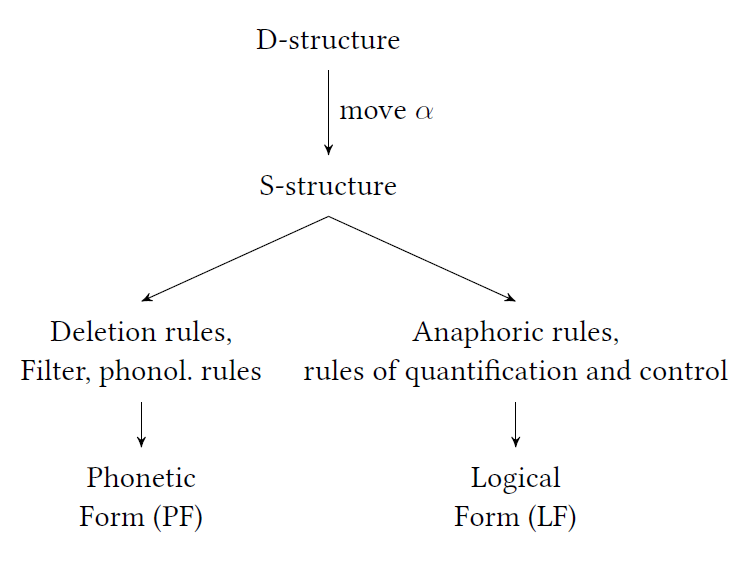
\includegraphics[scale=.43]{material/11tmodell}
%	\caption{T-Modell \citep[vgl.][]{MuellerS15b}}
%\end{figure}
%	
%\end{frame}

\begin{frame}
%\frametitle{T-Modell}

\begin{figure}
%\begin{tikzpicture}
%\node at (0,0) {D-structure};
%\draw[->] (0,-0.3)--(0,-1.5);
%\node[right] at (0,-0.9) {move $\alpha$};
%\node at (0,-1.8) {S-structure};
%\draw[->] (0,-2.1)--(-1.5-3);
%\draw[->] (0,-2.1)--(1.5,-3);
%\end{tikzpicture}
\begin{forest}
	sm edges,
	[D-structure, [S-structure,edge label={node[midway,right]{move $\alpha$} }
		[{Deletion rules,}\\{Filter, phonol. rules} [Phonetic Form (PF)], align=center]
		[{Anaphoric rules,}\\{rules of quantification and control}, align=center [Logical Form (LF)] ]
	]]
\end{forest}
	\caption{T-Modell \citep[vgl.][]{MuellerS15b}}
\end{figure}

\end{frame}


%%%%%%%%%%%%%%%%%%%%%%%%%%%%%%%%%%
%%%%%%%%%%%%%%%%%%%%%%%%%%%%%%%%%%
\subsection{Funktionale Phrasen II}

\iftoggle{sectoc}{
	\frame{
		%\begin{multicols}{2}
		\frametitle{~}
		\tableofcontents[currentsubsection,subsubsectionstyle=hide]
		%\end{multicols}
	}
}

%%%%%%%%%%%%%%%%%%%%%%%%%%%%%%%%%%
\begin{frame}
\frametitle{Funktionale Phrasen II}

\begin{itemize}
	\item Bisher \ras Nebensatzstellung im Deutschen
	\item Wann kommt die NS-Stellung vor? \ras Complementizer!
	
	\eal
	\ex[]{(Ich denke,) \alertred{dass} Syntax Spaß machen sollte.}
	\ex[]{Syntax \alertred{sollte} Spaß machen.}
	\ex[]{(Ich frage mich,) \alertred{ob} der Winter jemals enden wird.}
	\ex[]{Der Winter \alertred{wird} niemals enden.}
	\ex[*]{Der Winter \alertred{ob wird} niemals enden.}
	\zl
	
	\item Complementizer und finite Verben (in V2- und V1-Sätzen) sind \textbf{komplementär}!
	
\end{itemize}

\end{frame}


%%%%%%%%%%%%%%%%%%%%%%%%%%%%%%%%%%
%%%%%%%%%%%%%%%%%%%%%%%%%%%%%%%%%%
\subsubsection{Complementizer Phrase}
%\frame{
%\frametitle{~}
%	\tableofcontents[currentsection]
%}

%%%%%%%%%%%%%%%%%%%%%%%%%%%%%%%%%%
\begin{frame}
\frametitle{Complementizer Phrase (CP)}

\begin{itemize}
	\item C nimmt eine IP als Komplement
\end{itemize}

\begin{minipage}[b]{0.45\textwidth}
\begin{figure}
	\centering
	\scalebox{.6}{
		\begin{forest}
		sm edges,
		[IP [DP [Peter,roof]]
			[\MyPxbar{I} [VP 
					[\MyPxbar{V} [DP [den Wagen,roof]]
						[\zerobar{V} [gekauft]]
						]]
				[I [hat]]
				]
		]
		\end{forest}
		}
		\caption{NS als IP}	
\end{figure}		
\end{minipage}  
  	%  
\pause
	%
\begin{minipage}[b]{0.45\textwidth}
\begin{figure}
	\centering
	\scalebox{.6}{
		\begin{forest}
		sm edges,
[CP	[\MyPxbar{C}	[\zerobar{C} [\alertred{dass}\\ \alertred{ob}\\ \alertred{weil}]]	
		[IP [DP [Peter,roof]]
			[\MyPxbar{I} [VP
					[\MyPxbar{V} [DP [den Wagen,roof]]
						[\zerobar{V} [gekauft]]
						]]
				[\zerobar{I} [\alert{hat}]]
				]
		]
	]
]
		\end{forest}
		}
		\caption{NS als CP}	
\end{figure}		
\end{minipage}  

\nocite{Fries&MyP16i}

\end{frame}


%%%%%%%%%%%%%%%%%%%%%%%%%%%%%%%%%%
\begin{frame}
\frametitle{Complementizer Phrase}

\begin{itemize}
	\item Die CP ist für den Satzmodus zuständig.
	\begin{itemize}
		\item Eingebetteter Satz
		\item Eingebetteter Fragesatz
		\item Deklarativsatz
		\item E- oder K-Fragesatz
		\item Imperativsatz
	\end{itemize}
\end{itemize}
\end{frame}


%%%%%%%%%%%%%%%%%%%%%%%%%%%%%%%%%%
\begin{frame}
%\frametitle{Complementizer Phrase}

\begin{itemize}
	\item Die CP bestimmt die \textbf{Form} der IP. \ras Finit!
\end{itemize}

\begin{figure}[b]

	\begin{minipage}[b]{0.45\textwidth}
	\centering
	\tiny{
		\begin{forest}
		sm edges,
[*CP	[\MyPxbar{C}	[\zerobar{C} [dass]]
		[IP [DP [Peter,roof]]
			[\MyPxbar{I} [VP 
					[\MyPxbar{V} [DP [den Wagen,roof]]
						[\zerobar{V} [\alert{kaufen}]]{\draw[<-,red] (.south east)--++(0em,-1.5ex)--++(+3em,0pt)
node[anchor=west,align=center]{infinit};}
						]]
				[\zerobar{I} [$\emptyset$]]
				]
		]
	]
]		
		\end{forest}
		}
		\caption{Ungrammatisch}	
  	\end{minipage}  
  	%  
	%
	\begin{minipage}[b]{0.45\textwidth}
	\centering
	\tiny{
		\begin{forest}
		sm edges,
[CP	[\MyPxbar{C}	[\zerobar{C} [dass]]	
		[IP [DP [Peter,roof]]
			[\MyPxbar{I} [VP 
					[\MyPxbar{V} [DP [den Wagen,roof]]
						[\zerobar{V} [t$_{i}$]]
						]]
				[\zerobar{I} [\alert{kauft}$_{i}$]]{\draw[<-,red] (.south east)--++(0em,-1.5ex)--++(+2em,0pt)
node[anchor=west,align=center]{finit};}
				]
		]
	]
]
		\end{forest}
		}
		\caption{Grammatisch}	
  	\end{minipage}  

\end{figure}

\end{frame}


%%%%%%%%%%%%%%%%%%%%%%%%%%%%%%%%%%
\begin{frame}
%\frametitle{Complementizer Phrase}

\begin{itemize}
	\item Korrelation zwischen \textbf{Verbzweit- und Verbletztstruktur}
	\item Kopfbewegung
\end{itemize}


\begin{minipage}[b]{0.49\textwidth}
\begin{figure}
	\centering
	\tiny{
		\begin{forest}
		sm edges,
[CP	[\MyPxbar{C}	[\zerobar{C} [\alert{dass}]]{\draw[<-,red] (.south west)--++(0em,-2.5ex)--++(-1.5em,0pt)
node[anchor=east,align=center]{besetzt! \ras \\ keine I-C-Bewegung};}
		[IP [DP [Peter,roof]]
			[\MyPxbar{I} [VP 
					[\MyPxbar{V} [DP [den Wagen,roof]]
						[\zerobar{V} [t$_{i}$]]
						]]
				[\zerobar{I} [\alert{kauft$_{i}$}]]
				]
		]
	]
]		
		\end{forest}
		}
		\caption{V-I-Bewegung}	
\end{figure}		
\end{minipage}  
%  
%
\begin{minipage}[b]{0.49\textwidth}
\begin{figure}
	\centering
	\tiny{
		\begin{forest}
		sm edges,
[CP	[\MyPxbar{C}	[\zerobar{C} [\alert{kauft$_{i}$}]]{\draw[<-,red] (.south west)--++(0em,-2.5ex)--++(-1.5em,0pt)
node[anchor=east,align=center]{frei! \ras \\ I-C-Bewegung};}
		[IP [DP [Peter,roof]]
			[\MyPxbar{I} [VP 
					[\MyPxbar{V} [DP [den Wagen,roof]]
						[\zerobar{V} [t$_{i}$]]
						]]
				[\zerobar{I} [\alert{t$_{i}$}]]
				]
		]
	]
]
		\end{forest}
		}
		\caption{V-I-C-Bewegung}
\end{figure}			
\end{minipage}  

\end{frame}


%%%%%%%%%%%%%%%%%%%%%%%%%%%%%%%%%%
\begin{frame}

\begin{itemize}
	\item \textbf{Weitere Position} für Verbzweitsätze \ras aber \textbf{nur eine} Phrasenposition
\ea[*]{[Den Wagen] [Peter] kauft gestern.}
\z

\end{itemize}

\begin{figure}[b]

	\begin{minipage}[b]{0.49\textwidth}
	\centering
	\scalebox{.55}{
		\begin{forest}
		sm edges,
[CP	[\alert{DP$_{i}$} [Peter,roof]]{\draw[<-,red] (.south west)--++(0em,-1.5ex)--++(-2em,0pt)
node[anchor=east,align=center]{Phrase};}
	[\MyPxbar{C}	[\zerobar{C} [kauft$_{ii}$]]
		[IP [\alert{t$_{i}$}]
			[\MyPxbar{I} [VP 
					[\MyPxbar{V} [DP [den Wagen,roof]]
						[\zerobar{V} [t$_{ii}$]]
						]]
				[\zerobar{I} [t$_{ii}$]]
				]
		]
	]
]		
		\end{forest}
		}
		\caption{Subjektbewegung}	
  	\end{minipage}  
%%
\pause
%%
	\begin{minipage}[b]{0.49\textwidth}
	\centering
	\scalebox{.55}{
		\begin{forest}
		sm edges,
[CP	[\alert{DP$_{ii}$} [den Wagen,roof]]{\draw[<-,red] (.south west)--++(0em,-1.5ex)--++(-2em,0pt)
node[anchor=east,align=center]{Phrase};}
	[\MyPxbar{C}	[\zerobar{C} [kauft$_{i}$]]
		[IP [DP [Peter,roof]]
			[\MyPxbar{I} [VP 
					[\MyPxbar{V} [\alert{t$_{ii}$}]
						[\zerobar{V} [t$_{i}$]]
						]]
				[\zerobar{I} [t$_{i}$]]
				]
		]
	]
]
		\end{forest}
		}
		\caption{Objektbewegung}	
  	\end{minipage}  
    
\end{figure}

\end{frame}


%%%%%%%%%%%%%%%%%%%%%%%%%%%%%%%%%%
\begin{frame}
\frametitle{Complementizer Phrase}

\begin{itemize}
	\item Die CP ist für den \textbf{Satzmodus} und die \textbf{illokutionäre Kraft} zuständig.
\end{itemize}

\begin{figure}[b]

	\begin{minipage}[b]{0.45\textwidth}
	\centering
	\scriptsize{
		\begin{forest}
		MyP edges,
		[CP [$\emptyset$]{\draw[<-,red] (.south west)--++(0em,-1.5ex)--++(-2em,0pt)
node[anchor=east,align=center]{leer};}
			[C' [C [dass]]{\draw[<-,red] (.south west)--++(0em,-1.5ex)--++(-2em,0pt)
node[anchor=east,align=center]{Subjunktion};}
				[IP [Peter den Wagen kauft,roof]]]]
		\end{forest}
		}
		\caption{Eingebetteter Satz}	
  	\end{minipage}  
%  
\pause            
%         
  	\begin{minipage}[b]{0.45\textwidth}
	\centering
	\scriptsize{
		\begin{forest}
		MyP edges,
		[CP [$\emptyset$]{\draw[<-,red] (.south west)--++(0em,-1.5ex)--++(-2em,0pt)
node[anchor=east,align=center]{leer};}
			[C' [C [kauft$_{i}$]]{\draw[<-,red] (.south west)--++(0em,-1.5ex)--++(-2em,0pt)
node[anchor=east,align=center]{Verb};}
				[IP [Peter den Wagen t$_{i}$,roof]]]]
		\end{forest}
		}
		\caption{Entscheidungsfrage}
  	\end{minipage}  
  	
\end{figure}

\end{frame}


%%%%%%%%%%%%%%%%%%%%%%%%%%%%%%%%%%
\begin{frame}
\frametitle{Complementizer Phrase}

\begin{itemize}
	\item Die CP ist für den \textbf{Satzmodus} und die \textbf{illokutionäre Kraft} zuständig.
\end{itemize}

\begin{figure}[b]

	\begin{minipage}[b]{0.45\textwidth}
	\centering
	\scriptsize{
		\begin{forest}
		MyP edges,
		[CP [DP$_{ii}$ [was,roof]]{\draw[<-,red] (.south west)--++(0em,-1.5ex)--++(-2em,0pt)
node[anchor=east,align=center]{W-Wort};}
			[C' [C [kauft$_{i}$]]{\draw[<-,red] (.south west)--++(0em,-1.5ex)--++(-2em,0pt)
node[anchor=east,align=center]{Verb};}
				[IP [Peter t$_{ii}$ t$_{i}$,roof]]]]
		\end{forest}
		}
		\caption{Konstituentenfrage}	
  	\end{minipage}  
  	%  
  	\pause            
  	%         
  	\begin{minipage}[b]{0.49\textwidth}
	\centering
	\scriptsize{
		\begin{forest}
		MyP edges,
		[CP [DP$_{ii}$ [Den Wagen,roof]]{\draw[<-,red] (.south west)--++(0em,-1.5ex)--++(-2em,0pt)
node[anchor=east,align=center]{Konstituente};}
			[C' [C [kauft$_{i}$]]{\draw[<-,red] (.south west)--++(0em,-1.5ex)--++(-2em,0pt)
node[anchor=east,align=center]{Verb};}
				[IP [Peter t$_{ii}$ t$_{i}$,roof]]]]
		\end{forest}
		}
		\caption{Aussagesatz}
  	\end{minipage}  
  
\end{figure}

\end{frame}


%%%%%%%%%%%%%%%%%%%%%%%%%%%%%%%%%%
%%%%%%%%%%%%%%%%%%%%%%%%%%%%%%%%%%
\subsection{Erklärungspotential}

\iftoggle{sectoc}{
	\frame{
		%\begin{multicols}{2}
		\frametitle{~}
		\tableofcontents[currentsubsection,subsubsectionstyle=hide]
		%\end{multicols}
	}
}

%%%%%%%%%%%%%%%%%%%%%%%%%%%%%%%%%%%
\begin{frame}
\frametitle{Erklärungspotential}

\begin{itemize}
	\item Warum ist eine \textbf{VP mit Subjekt} nicht möglich?
	\eal 
	\ex[]{\dots\ (dass) [Peter den Wagen \alertred{kauft}]$_{IP}$.}
	\ex[*]{\dots\ (dass) [Peter den Wagen \alertred{kaufen}]$_{VP}$.}
	\zl

\pause
	\begin{itemize}
		\item \textbf{Kasus} und \textbf{$\theta$-Rolle} werden \textbf{strukturell} vergeben.
		\item[]
		\item Erst durch die \textbf{Subjekt-Verb-Kongruenz} erhält das Subjekt \textsc{nom}-Kasus.
		\item[]
		\item Subjekt-Verb-Kongruenz geschieht durch die \textbf{SpecIP-I$^{0}$-Relation} (strukturelle/lokale Relation).
	\end{itemize}
\end{itemize}		

\end{frame}


%%%%%%%%%%%%%%%%%%%%%%%%%%%%%%%%%%%
\begin{frame}

\begin{itemize}
	\item Warum ist eine \textbf{VP mit Subjekt} nicht möglich?
	\eal 
	\ex[]{\dots\ (dass) [Peter den Wagen \alertred{kauft}]$_{IP}$.}
	\ex[*]{\dots\ (dass) [Peter den Wagen \alertred{kaufen}]$_{VP}$.}
	\zl

\end{itemize}

\begin{figure}[b]
%	\begin{minipage}[b]{0.80\textwidth}
	\centering
	\scriptsize{
		\begin{forest}
		MyP edges,
		[IP 
			[DP [Peter,roof]]{\draw[<-,red] (.north west)--++(0em,+1.5ex)--++(-2em,0pt)
node[anchor=east,align=center]{\textsc{agens}- \& \\ \textsc{akk}-Vergabe};}
			[\MyPxbar{I} 
				[VP 					
					[\MyPxbar{V} 
						[DP [den Wagen,roof]]{\draw[<-,red] (.north west)--++(0em,+1.5ex)--++(-2em,0pt)
node[anchor=east,align=center]{\textsc{patiens}- \& \\ \textsc{akk}-Vergabe};}
						[\zerobar{V} [gekauft]]
					]
				]
				[\zerobar{I} [hat]]
			]
		]
		\end{forest}
		}
	\caption{Position und Funktion im X-Bar-Schema} 
%  	\end{minipage}  
 
\end{figure}

\end{frame}


%%%%%%%%%%%%%%%%%%%%%%%%%%%%%%%%%%%
\begin{frame}
\frametitle{Erklärungspotential}


\begin{itemize}
	\item Warum ist die \textbf{Vorfeldbesetzung durch VP mit Subjekt} nicht möglich?
	\eal 
	\ex[]{[Den Wagen \alertred{gekauft}]$_{VP}$ hat Peter gestern.}
	\ex[*]{[Peter den Wagen \alertred{gekauft}]$_{VP}$ hat gestern.}
	\zl

\pause
	\item Damit das Subjekt sichtbar (overt realisiert) wird, muss es \textbf{in SpecIP} \textsc{nom} \textbf{erhalten} \ras Es ist nicht (mehr) in der VP!

\end{itemize}		

\pause
\begin{itemize}
	\item \textbf{Gewinn} \ras Elegante und restriktive Theorie \nocite{Haspelmath94a}

	\begin{itemize}
		\item Keine \textbf{Köpfe} ohne Phrasen
		\item Keine \textbf{Phrasen} ohne Köpfe (exozentrische Phrasen)
		\item Strukturelle \textbf{Position} bestimmt Funktion
		\item \textbf{Einheitlichkeit} der X-Bar-Struktur
	\end{itemize}		

\end{itemize}

\end{frame}


%%%%%%%%%%%%%%%%%%%%%%%%%%%%%%%%%%%
\begin{frame}

\begin{itemize}
	\item \textbf{Grammatikalisierung} \ras ein seltenes Argument \citep{Haspelmath94a}
	\item Hilfsverben, Tempus- und Aspektaffixe werden \textbf{aus Vollverben} grammatikalisiert \ras \textbf{Unterschied zwischen Wort oder Affix} ist nicht von Bedeutung.
	\item Die \textbf{Kopf-Dependent-Relation} bleibt bei der Grammatikalisierung immer erhalten \ras Hilfsverben und weitere Affixe sind Köpfe.
\end{itemize}


\begin{figure}[b]

	\begin{minipage}[b]{0.40\textwidth}
	\centering
	\scalebox{.8}{
		\begin{forest}
		MyP edges,
		[VP [DP [Julia,roof]]
			[\MyPxbar{V} [VP [cantare,roof]]
				[\zerobar{V} [\alert{habet}]]		{\draw[<-,red] (.south east)--++(0em,-1.5ex)--++(+2em,0pt)
node[anchor=west,align=center]{Kopf};}
			]
		]
		\end{forest}
		}
		\caption{Latein}	
  	\end{minipage}  
  	%  
  	\pause            
  	%         
  	\begin{minipage}[b]{0.40\textwidth}
	\centering
	\scalebox{.8}{
		\begin{forest}
		MyP edges,
		[IP [DP [Julia,roof]]
			[\MyPxbar{I} [VP [cant-,roof]]
				[\zerobar{I} [\alert{-ará}]]{\draw[<-,red] (.south east)--++(0em,-1.5ex)--++(+2em,0pt)
node[anchor=west,align=center]{Kopf};}
			]
		]
		\end{forest}
		}
		\caption{Spanisch}
  	\end{minipage}  
  	
\end{figure}


\end{frame}


%%%%%%%%%%%%%%%%%%%%%%%%%%%%%%%%%%
%%%%%%%%%%%%%%%%%%%%%%%%%%%%%%%%%%
\subsection{Mehr funktionale Kategorien}

\iftoggle{sectoc}{
	\frame{
		%\begin{multicols}{2}
		\frametitle{~}
		\tableofcontents[currentsubsection,subsubsectionstyle=hide]
		%\end{multicols}
	}
}


%%%%%%%%%%%%%%%%%%%%%%%%%%%%%%%%%%%
%\begin{frame}
%\frametitle{Mehr funktionale Kategorien}
%\nocite{Lenerz93a}
%
%\begin{figure}[b]
%	\begin{minipage}[b]{0.48\textwidth}
%		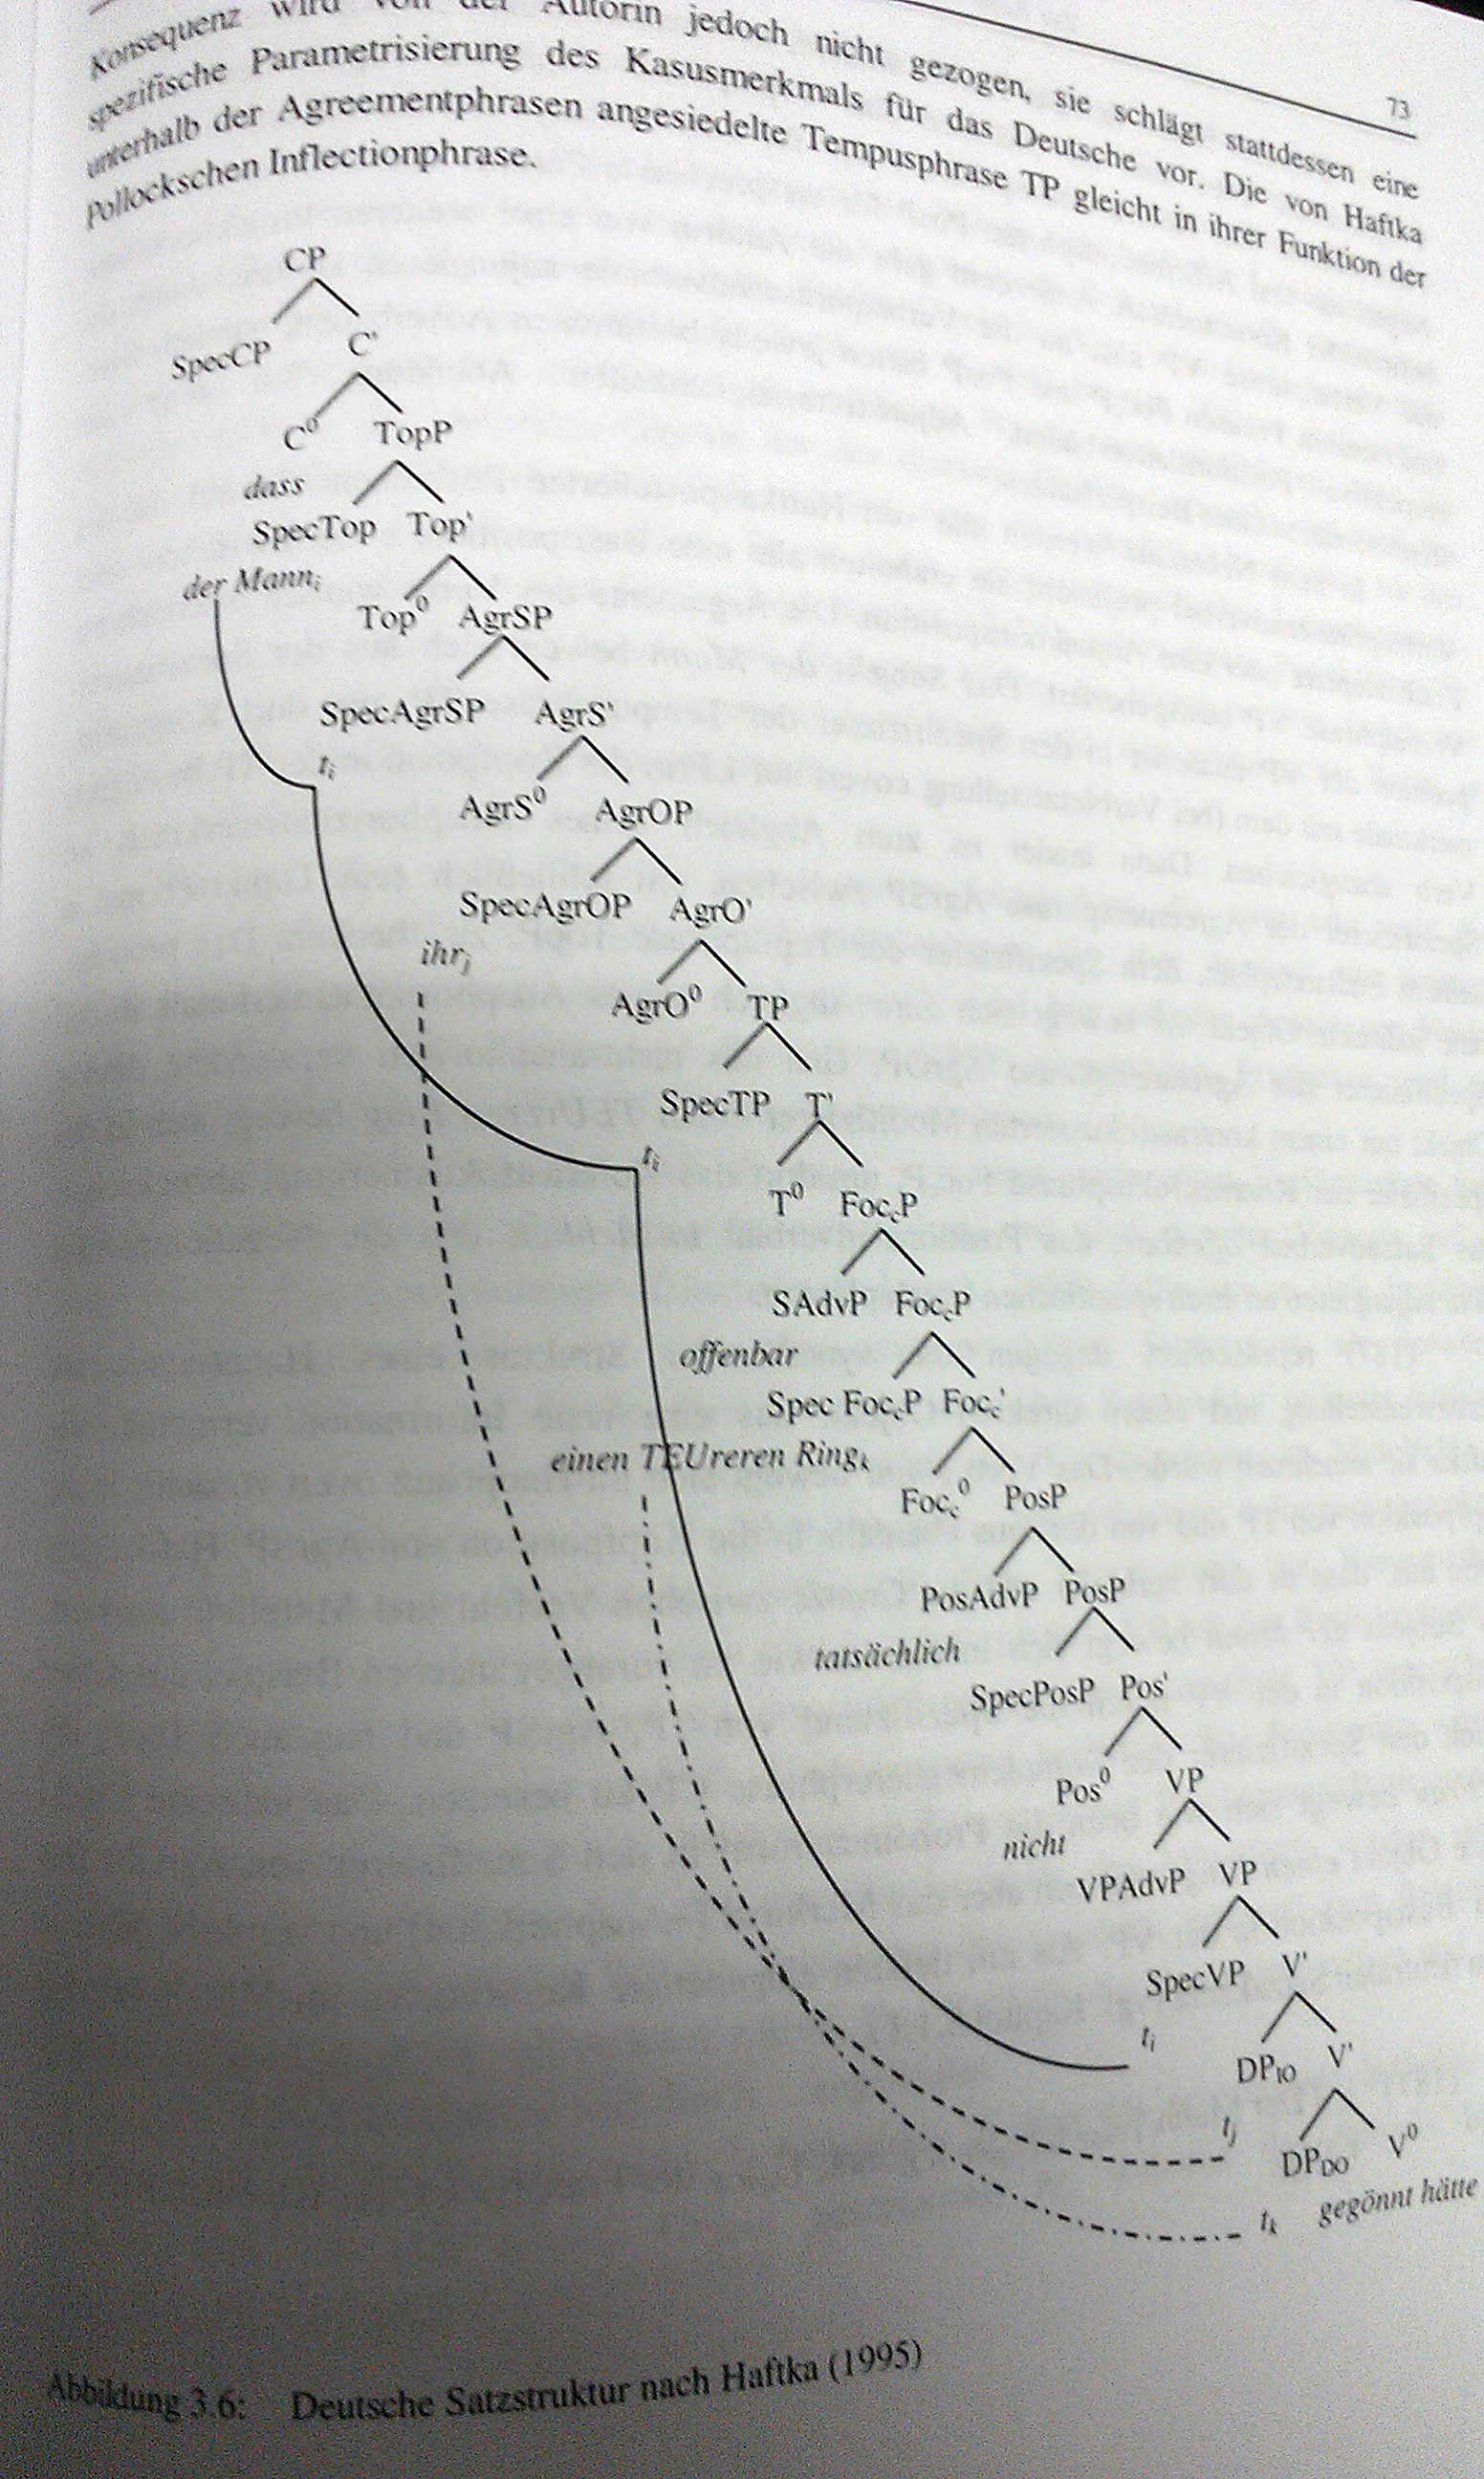
\includegraphics[scale=0.06]{material/Haftka95CP}
%		\caption{CP-Struktur (Haftka 1995)}
%		%\label{Zeichen1}
%	\end{minipage}
%	%
%	%				
%	\begin{minipage}[b]{0.48\textwidth}
%		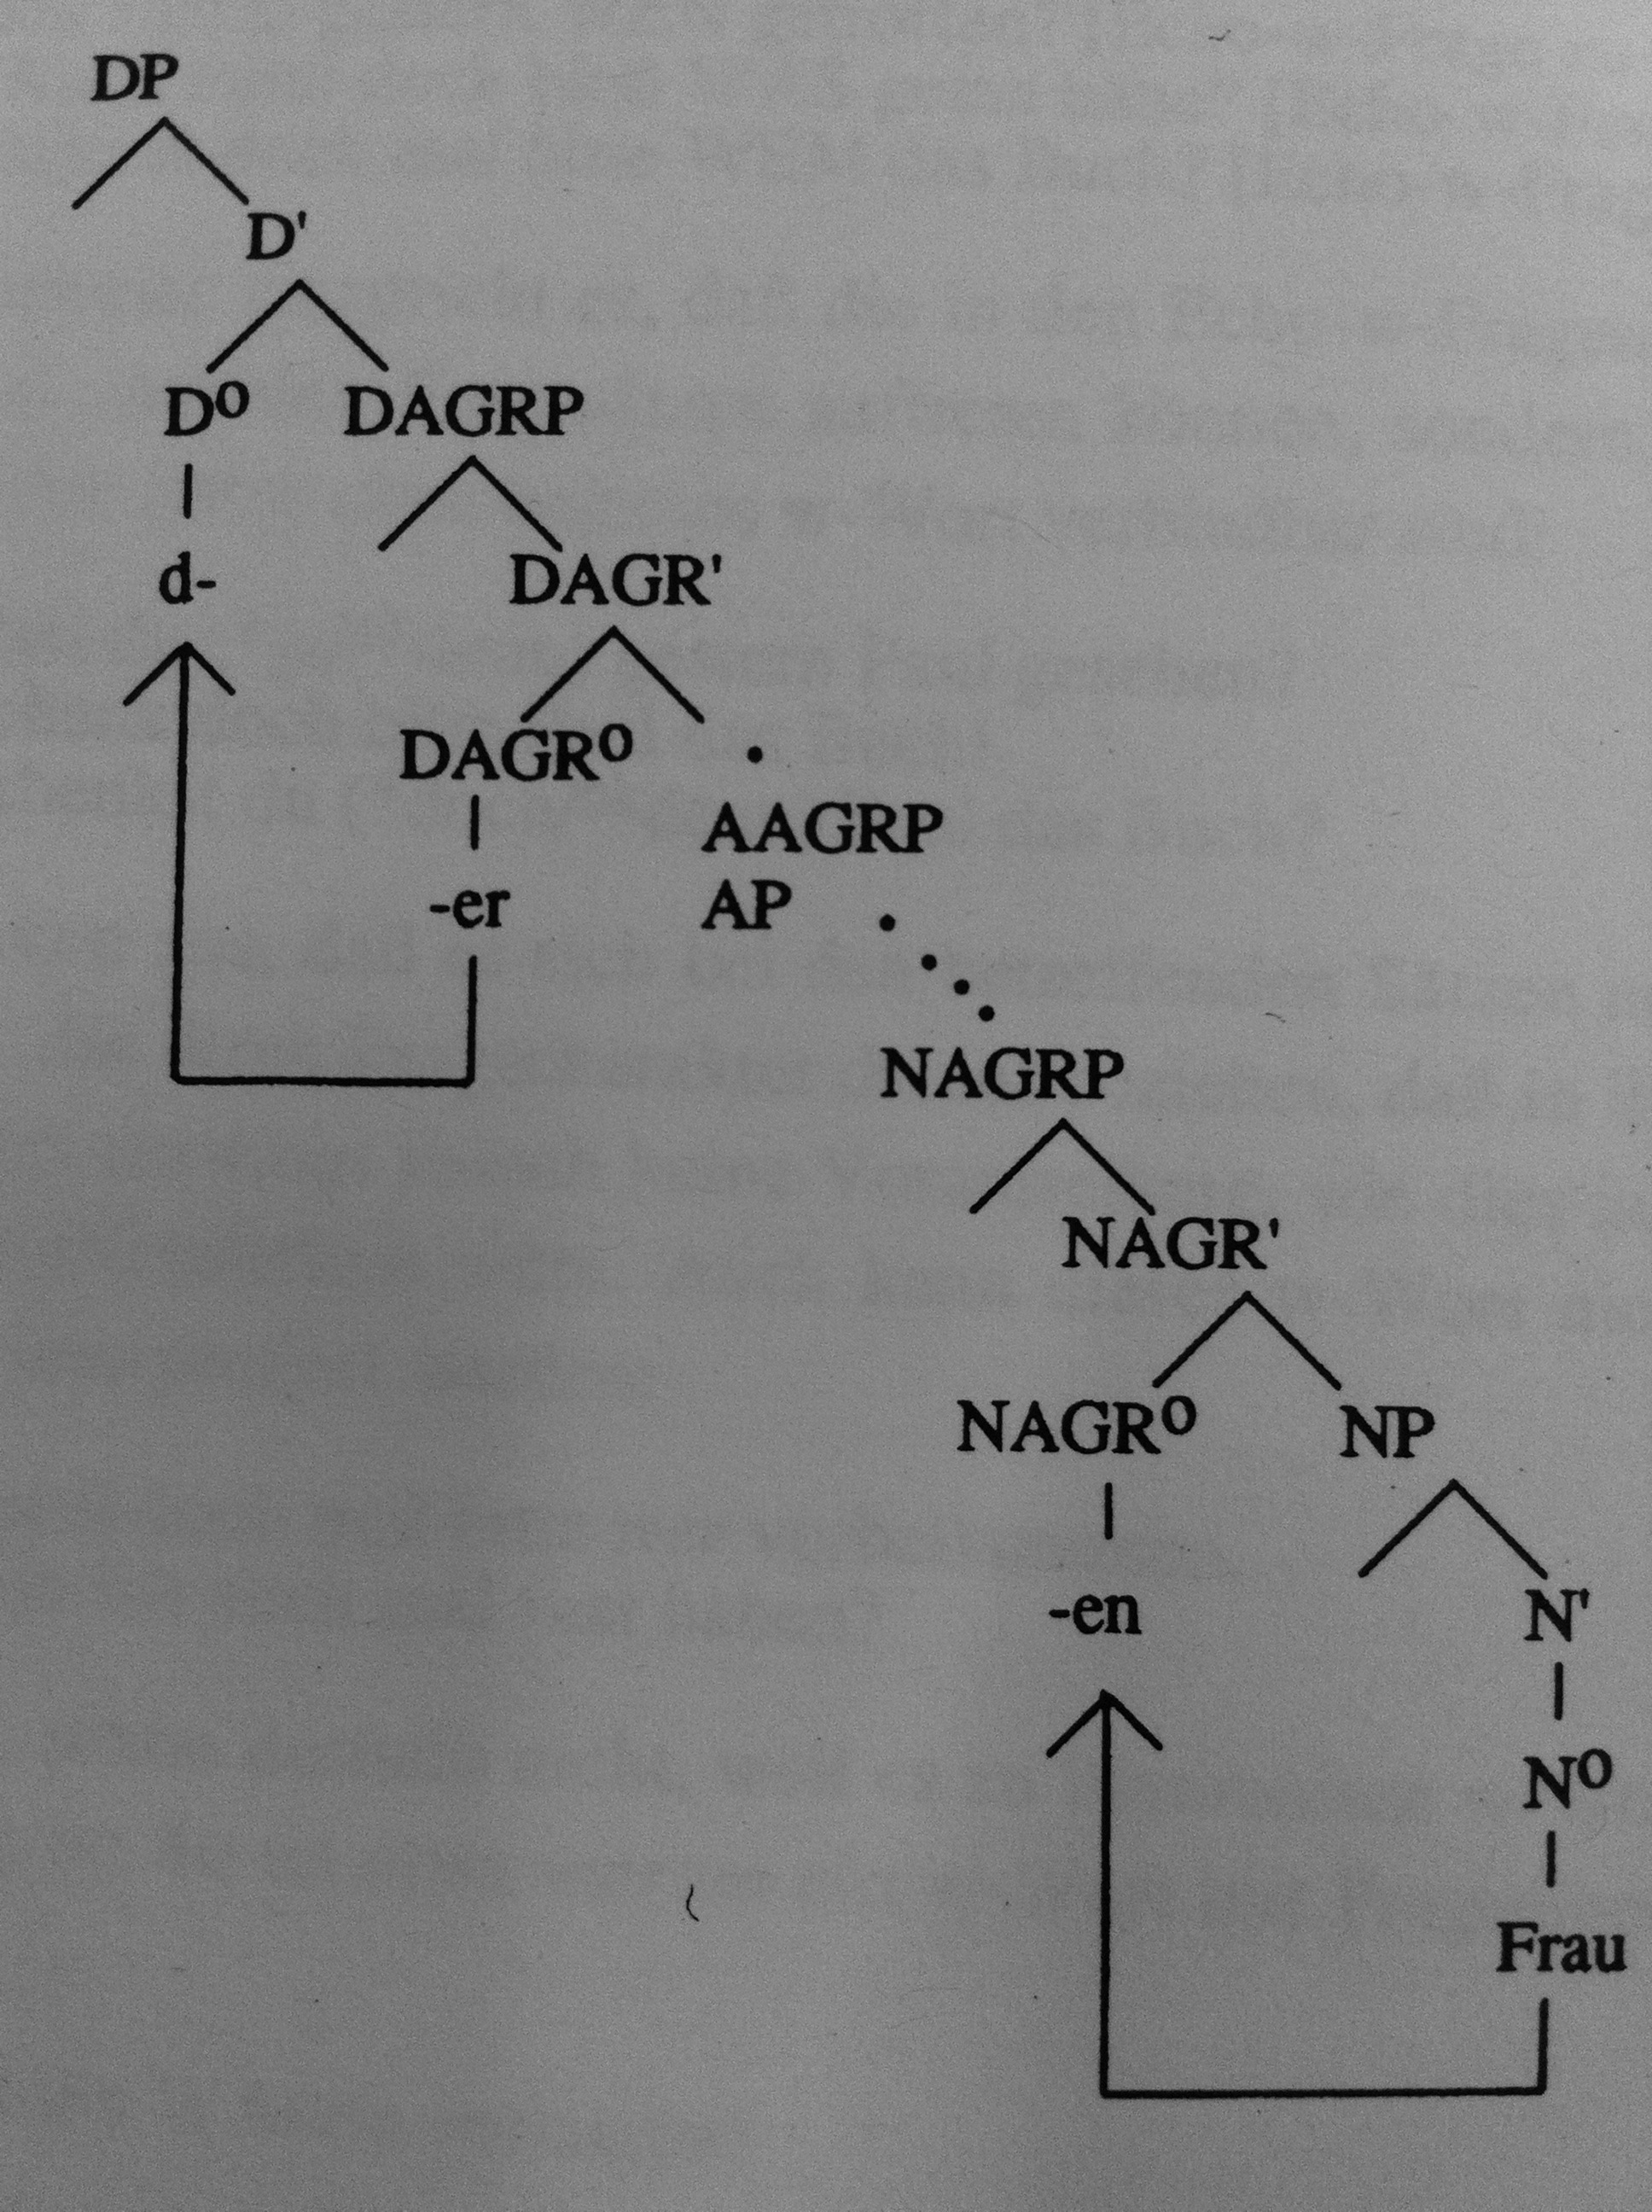
\includegraphics[scale=0.06]{material/Lenerz93DP}
%		\caption{DP-Struktur \citep{Lenerz93a}}
%		%\label{Zeichen2}
%	\end{minipage}                        
%\end{figure}
%
%\end{frame}


\begin{frame}
\nocite{Lenerz93a}

	\begin{minipage}[c]{0.48\textwidth}
\begin{figure}
	\centering
	\scalebox{.45}{\begin{forest}MyP edges,
			[DP
			[]
			[D'
				[\zerobar{D} [d-, name=d] ]
				[DAGRP
					[]
					[DAGRP'
						[\zerobar{DAGRP} [-er, name=er] ]
						[{AAGRP}\\{AP}, align=center [NAGRP, edge=dotted
						[]
						[NAGR'
							[\zerobar{NAGR} [-en, name=en] ]
							[NP
								[]
								[N' [\zerobar{N} [Frau, name=Frau] ] ]
							]
						]
						] ]
					]
			]
			] ]{
			\draw[->] (Frau) to [out=south west, in=south] (en.south);
			\draw[->] (er) to [out=south west, in=south] (d.south);}
		\end{forest}}
	\caption{DP-Struktur \citep{Lenerz93a}}
\end{figure}
	\end{minipage}
	%
	%				
	\begin{minipage}[c]{0.48\textwidth}
\begin{figure}
			\centering 
			\scalebox{.19}{	\begin{forest}
				[CP
					[SpecCP]
					[C'
						[{\zerobar{C}}\\{dass}, align=center]
						[TopP
							[SpecTop \\ \textit{der Mann\textsubscript{i}}, align=center, name=Mann]
							[Top'
								[\zerobar{Top}]
								[AgrSP
									[SpecAgrSP \\ t\textsubscript{i}, align=center, name=Agr]
									[AgrS'
										[\zerobar{AgrS}]
										[AgrOP
											[SpecAgrOP \\ \textit{ihr\textsubscript{j}}, align=center, name=ihr]
											[AgrO'
												[\zerobar{AgrO}]
												[TP
													[SpecTP \\ t\textsubscript{i}, align=center, name=i1]
													[T'
														[\zerobar{T}]
														[Foc\textsubscript{c}P
															[SAdvP\\ \textit{offenbar}, align=center]
															[Foc\textsubscript{c}P
															[SpecFoc\textsubscript{c}P \\ \textit{einen TEUeren Ring\textsubscript{k}}, align=center, name=ring]
															[Foc\textsubscript{c}'
																[\zerobar{Foc\textsubscript{c}}]
																[PosP
																	[PosAdvP \\ \textit{tatsächlich}, align=center]
																	[PosP
																		[SpecPosP]
																		[Pos'
																			[\zerobar{Pos}\\nicht, align=center]
																			[VP	
																				[VPAdvP]
																				[VP
																					[SpecVP\\ t\textsubscript{i}, align=center, name=i2]
																					[V'
																						[DP\textsubscript{IO} \\ t\textsubscript{j}, align=center, name=j]
																						[V'
																							[DP\textsubscript{DO} \\ t\textsubscript{k}, align=center, name=k]
																							[\zerobar{V}\\\textit{gegönnt hätte}, align=center]
																						]
																					]
																				]
																			]
																		]
																	]
																]
																]
															]	
															]
														]
													]			
												]
											]
										]
									]
								]
							]
						]
					]
					{\draw (i2) to [out=south west, in=south] (i1) to [out=south west, in=south] (Agr) to [out=south west, in=south] (Mann);
				\draw[dashed, thick] (j) to [out=south west, in=south] (ihr);
					\draw[dotted, thick] (k) to [out=south west, in=south] (ring);
				}
			\end{forest}}
		\caption{CP-Struktur (Haftka 1995)}
		\end{figure}
	\end{minipage}                        

\end{frame}

%%%%%%%%%%%%%%%%%%%%%%%%%%%%%%%%%%
%%%%%%%%%%%%%%%%%%%%%%%%%%%%%%%%%%
\subsection{Übung}

\iftoggle{sectoc}{
	\frame{
		%\begin{multicols}{2}
		\frametitle{~}
		\tableofcontents[currentsubsection,subsubsectionstyle=hide]
		%\end{multicols}
	}
}


%%%%%%%%%%%%%%%%%%%%%%%%%%%%%%%%%%%
%%%%%%%%%%%%%%%%%%%%%%%%%%%%%%%%%%%

%%%%%%%%%%%%%%%%%%%%%%%%%%%%%%%%%%%
\begin{frame}
\frametitle{Übung}

\begin{itemize}
		\item Erklären Sie mithilfe des X-Bar-Schemas die \textbf{Ambiguität} im folgenden Satz:
	
		\ea Das Kind küsst die Mama.
		\z

\end{itemize}
\end{frame}


%%%%%%%%%%%%%%%%%%%%%%%%%%%%%%%%%%%

\iftoggle{ue-loesung}{

%%%%%%%%%%%%%%%%%%%%%%%%%%%%%%%%%%%
%06f Syntax ue-loesung01
%%%%%%%%%%%%%%%%%%%%%%%%%%%%%%%%%

\begin{frame}
\frametitle{Übung -- Lösung}


\begin{minipage}[b]{0.29\textwidth}
	\centering
	\scalebox{0.55}{
		\begin{forest}
			MyP edges,
			[CP
			[DP$ _{k} $[Das Kind, roof]]
			[\MyPxbar{C} 
			[\zerobar{C}[küsst$ _{i} $]]
			[IP
			[\alertgreen{t$_{k}$}]
			[\MyPxbar{I}
			[VP [\MyPxbar{V}
			[DP[die Mama, roof]]
			[\zerobar{V}[t$ _{i} $]]
			]
			]
			[\zerobar{I}[t$ _{i} $]]
			]
			]
			]
			]
		\end{forest}
		}
\end{minipage}
%
%
\begin{minipage}[b]{0.31\textwidth}
	\centering
	\scalebox{0.55}{
		\begin{forest}
			MyP edges,
			[CP
			[DP$ _{k} $[Das Kind, roof]]
			[\MyPxbar{C} 
			[\zerobar{C}[küsst$ _{i} $]]
			[IP
			[DP[die Mama, roof]]
			[\MyPxbar{I}
			[VP [\MyPxbar{V}
			[\alertgreen{t$_{k}$}]
			[\zerobar{V}[t$ _{i} $]]
			]
			]
			[\zerobar{I}[t$ _{i} $]]
			]
			]
			]
			]
		\end{forest}
		}
\end{minipage}
%%
%%
\begin{minipage}[b]{.38\textwidth}


\begin{itemize*}
	\alertgreen{\item {\small \MyPobj{das Kind} und \MyPobj{die Mama} sind im Akkusativ und im Nominativ formgleich (Synkretismus).}}
	\alertgreen{\item {\small Im Dt. kann eine Phrase in die SpecCP-Position bewegt werden.}}
	\alertgreen{\item {\small Wegen des Synkretismus' ist nicht ersichtlich, ob \MyPobj{das Kind} sich aus der SpecIP- oder aus der Schwesterposition von V\MyPup{0} bewegt hat. }}
\end{itemize*}

\end{minipage}
\end{frame}


}

%%%%%%%%%%%%%%%%%%%%%%%%%%%%%%%%%%%

\begin{frame}
\frametitle{Übung}

\begin{itemize}

	\item Erklären Sie mithilfe des X-Bar-Schemas, warum der folgende Satz \textbf{ungrammatisch} ist:
	
	\ea Im Auto ich habe heute geschlafen.
	\z
	
\end{itemize}
\end{frame}



%%%%%%%%%%%%%%%%%%%%%%%%%%%%%%%%%%%

\iftoggle{ue-loesung}{

%%%%%%%%%%%%%%%%%%%%%%%%%%%%%%%%%%%
%06f Syntax ue-loesung02
%%%%%%%%%%%%%%%%%%%%%%%%%%%%%%%%%

\begin{frame}
\frametitle{Übung -- Lösung}

\begin{minipage}[b]{0.45\textwidth}
	\centering
	\scalebox{0.6}{
		\begin{forest}
			MyP edges,
			[CP
			[DP$_{k}$ [Ich,roof]]
			[\MyPxbar{C} [\zerobar{C} [habe$_{i}$]]
			[IP [t$_{k}$]
			[\MyPxbar{I}
			[VP	[AdVP [heute,roof]]
			[VP [PP	[im Auto,roof]]{\draw[->,red] (.south west)--++(-7em,0em)--++(0em,14em)
				node[anchor=east,align=center]{PP kann nicht \\ bewegt werden};}
			[\MyPxbar{V} [\zerobar{V} [geschlafen t$_{i}$]]]
			]
			]
			[\zerobar{I} [t$_{i}$]]
			]
			]
			]	
			]
		\end{forest}
	}
\end{minipage}  
%            
%         
\begin{minipage}[b]{0.45\textwidth}
{\small 
	Nur eine Phrase, d.\,h.\ entweder die DP \MyPobj{ich} oder die PP \MyPobj{im Auto}, kann die SpecCP-Position belegen. Da die DP und die PP zusammen nicht eine Phrase bilden, können nicht \textbf{beide} Phrasen in diese Position bewegt werden.
}
\end{minipage}  

\end{frame}
}

%%%%%%%%%%%%%%%%%%%%%%%%%%%%%%%%%%%

%%%%%%%%%%%%%%%%%%%%%%%%%%%%%%%%%%%
\begin{frame}
\frametitle{Übung}

\begin{itemize}
	\item Was ist an dieser Struktur misslungen? Beziehen Sie sich in Ihrer Antwort \ua auf die in der Sitzung behandelten Köpfigkeitsmerkmale und Strukturaufbaugesetzmäßigkeiten.
\end{itemize}

\begin{figure}
\scalebox{.75}{\begin{forest} sm edges,
		[S
			[VP [V [Tea] ] ]
			[NP
				[P [with]]
				[Det [some]]
				[N [lemon]]
			]
			[PP
				[P [tastes]]
				[NP [Adj [really] ] [N [nice]] ]
			]
		]
	\end{forest}}
%	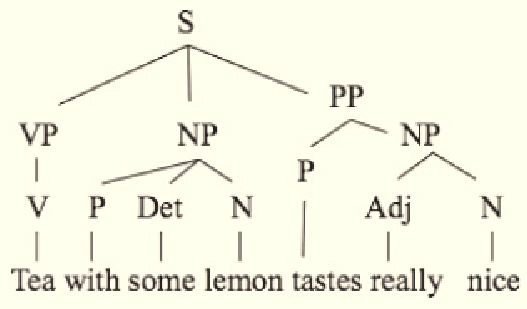
\includegraphics[scale=.45]{material/wrongtree}
	\caption{vgl.\ \url{http://specgram.com/CLXV.1/05.cruz-ferreira.know22.html}}
\end{figure}
	
\end{frame}



%%%%%%%%%%%%%%%%%%%%%%%%%%%%%%%%%%%

\iftoggle{ue-loesung}{
	
%%%%%%%%%%%%%%%%%%%%%%%%%%%%%%%%%%%
%06f Syntax ue-loesung03
%%%%%%%%%%%%%%%%%%%%%%%%%%%%%%%%%%%
	
\begin{frame}
\frametitle{Übung -- Lösung}


\begin{columns}

\begin{column}{.45\textwidth}
\begin{figure}
	\scalebox{.6}{\begin{forest} sm edges,
			[S
			[VP [V [Tea] ] ]
			[NP
			[P [with]]
			[Det [some]]
			[N [lemon]]
			]
			[PP
			[P [tastes]]
			[NP [Adj [really] ] [N [nice]] ]
			]
			]
	\end{forest}}
	%	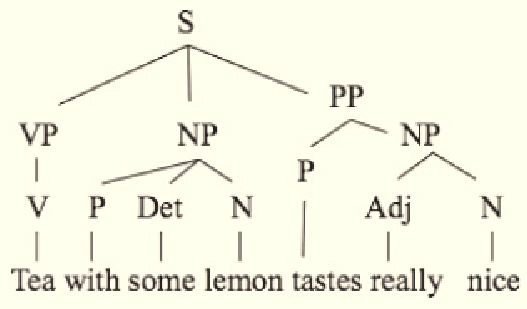
\includegraphics[scale=.45]{material/wrongtree}
	\caption{vgl.\ \url{http://specgram.com/CLXV.1/05.cruz-ferreira.know22.html}}
\end{figure}
\end{column}
%%
%%
\begin{column}{.55\textwidth}

\begin{itemize}
	\item keine binäre Struktur (mehr als zwei Töchter)
	\item falsche Kategorien bestimmt (\zB \MyPobj{Tea}: V?) 
	\item Es gibt Köpfe ohne Phrasen
	\item keine Zwischen Projektionen
	\item Satz ist exozentrisch
	\item \dots
\end{itemize}

\end{column}
\end{columns}

\end{frame}


}


%%%%%%%%%%%%%%%%%%%%%%%%%%%%%%%%%%
%%%%%%%%%%%%%%%%%%%%%%%%%%%%%%%%%%

\subsection{Hausaufgabe}

%%%%%%%%%%%%%%%%%%%%%%%%%%%%%%%%%%%
%%%%%%%%%%%%%%%%%%%%%%%%%%%%%%%%%%%

%%%%%%%%%%%%%%%%%%%%%%%%%%%%%%%%%%
\begin{frame}
\frametitle{Hausaufgabe}

\begin{itemize}
	\item Geben Sie an, um welchen \textbf{Phrasentyp} es sich bei den folgenden Phrasen handelt, und \textbf{welches Wort} sich in der \textbf{Kopfposition} der Phrasen befindet.
	
	\eal
	\ex viele besorgte Mütter
	\ex den Menschen in Not helfen
	\ex Wasser ohne Kohlensäure
	\ex auf Maria warten
	\ex ob sie heute kommen werden
	\ex Peter seine Traumfrau gefunden hat
	\zl
	
\end{itemize}

\end{frame}

%%%%%%%%%%%%%%%%%%%%%%%%%%%%%%%%%%%

%%%%%%%%%%%%%%%%%%%%%%%%%%%%%%%%%%
\begin{frame}
\frametitle{Hausaufgabe}

\begin{itemize}
	\item Analysieren Sie die folgenden Phrasen nach dem X-Bar-Schema (ohne Abkürzungen).

	\ea Peter schläft.
	\ex Wer schläft?
	\ex Hat sie dir die schwierige Frage nach den Spuren gestellt?
	\ex die fast vor dem Mittagessen erstellte Speisekarte
	\z

\end{itemize}
\end{frame}


%%%%%%%%%%%%%%%%%%%%%%%%%%%%%%%%%%%%%%%%%%%%

\iftoggle{ha-loesung}{

%%%%%%%%%%%%%%%
%06f Syntax ha-loesung
%%%%%%%%%%%%%%%%


\begin{frame}
\frametitle{Hausaufgabe -- Lösung}

\begin{itemize}
	\item Geben Sie an, um welchen \textbf{Phrasentyp} es sich bei den folgenden Phrasen handelt, und \textbf{welches Wort} sich in der \textbf{Kopfposition} der Phrasen befindet:
\end{itemize}	

\eal
	\ex viele besorgte Mütter  \pause \hfill \alertred{Mütter} \& \alertred{NP} oder \alertred{viele} \& \alertred{DP} \pause 

	\ex den Menschen in Not helfen \pause \hfill \alertred{helfen} \& \alertred{VP} \pause 
	
	\ex Wasser ohne Kohlensäure \pause \hfill \alertred{Wasser} \& \alertred{NP} oder \alertred{$\emptyset$} \& \alertred{DP} \pause 
	
	\ex auf Maria warten \pause \hfill \alertred{warten} \& \alertred{VP} \pause 
	
	\ex ob sie heute kommen werden \pause \hfill \alertred{ob} \& \alertred{CP} \pause 
	
	\ex Peter seine Traumfrau gefunden hat \pause \hfill \alertred{hat} \& \alertred{IP}
\zl

\end{frame}

%%%%%%%%%%%%%%%%%%%%%%%%%%%%%%%%%%%%%%

\begin{frame}
\frametitle{Hausaufgabe -- Lösung}

\begin{minipage}[b]{0.45\textwidth}
	
	{\small Peter schläft.}
	
	\pause
	
	\centering
	\scalebox{0.6}{
		\begin{forest}
			MyP edges,
			[CP 
			[DP$_{k}$ [Peter,roof]
			]
			[\MyPxbar{C}
			[\zerobar{C} [schläft$_{i}$]
			]
			[IP [t$_{k}$]
			[\MyPxbar{I}
			[VP [\MyPxbar{V} [\zerobar{V} [t$_{i}$	]]]]
			[\zerobar{I} [t$_{i}$]]
			]
			]
			]
			]
		\end{forest}
	}
\end{minipage}  
%            
%         
\begin{minipage}[b]{0.45\textwidth}
	
	\pause 
	
	{\small Wer schläft?}	
	
	\pause 
	
	\centering
	\scalebox{0.6}{
		\begin{forest}
			MyP edges,
			[CP 
			[DP$_{k}$ [Wer,roof]
			]
			[\MyPxbar{C}
			[\zerobar{C} [schläft$_{i}$]
			]
			[IP [t$_{k}$]
			[\MyPxbar{I}
			[VP [\MyPxbar{V} [\zerobar{V} [t$_{i}$	]]]]
			[\zerobar{I} [t$_{i}$]]
			]
			]
			]
			]
		\end{forest}
	}
\end{minipage}  

\end{frame}


%%%%%%%%%%%%%%%%%%%%%%%%%%%%%%%%%%
\begin{frame}
\frametitle{Hausaufgabe -- Lösung}

{\small Hat sie dir die schwierige Frage nach den Spuren gestellt?}

\pause

\begin{minipage}[b]{0.45\textwidth}

\centering
\scalebox{0.6}{
	\begin{forest}
		MyP edges,
		[CP 
		[\MyPxbar{C}
		[\zerobar{C} [Hat$_{i}$]
		]
		[IP [DP [\MyPxbar{D} [\zerobar{D} [sie]]]
		]
		[\MyPxbar{I}
		[VP 
		[DP [\MyPxbar{D} [\zerobar{D} [dir]]]]
		[\MyPxbar{V} 								
		[DP, draw, red 
		[die \dots\ Spuren,roof]
		]		
		[\zerobar{V} [gestellt]]
		]
		]
		[\zerobar{I} [t$_{i}$]]
		]
		]
		]
		]
	\end{forest}
}
\end{minipage}  
%      
\pause  	      
%         
\begin{minipage}[b]{0.45\textwidth}

\centering
\scalebox{0.4}{
	\begin{forest}
		MyP edges,
		[DP
		[\MyPxbar{D}
		[\zerobar{D}[die]]
		[NP
		[AP [\MyPxbar{A} [\zerobar{A} [schwierige]]]]
		[NP 
		[\MyPxbar{N} 
		[\zerobar{N} [Frage]]
		[PP
		[\MyPxbar{P} 
		[\zerobar{P} [nach]]
		[DP
		[\MyPxbar{D}
		[\zerobar{D} [den]]
		[NP [\MyPxbar{N} [\zerobar{N} [Spuren]]]]
		]
		]
		]
		]
		]
		]
		]
		]
		]
	\end{forest}
}
\end{minipage}  

\end{frame}


%%%%%%%%%%%%%%%%%%%%%%%%%%%%%%%%%%
\begin{frame}
\frametitle{Hausaufgabe -- Lösung}

{\small die fast vor dem Mittagessen erstellte Speisekarte}

\pause 

\begin{minipage}[b]{0.45\textwidth}

\centering
\scalebox{0.6}{
\begin{forest}
	MyP edges,
	[DP
	[\MyPxbar{D}
	[\zerobar{D}[die]]
	[NP
	[AP
	[PP, draw, red 
	[fast vor dem Mittagessen,roof]
	%							[AdvP [\MyPxbar{Adv} [\zerobar{Adv} [kurz]]]]
	%							[PP [\MyPxbar{P}
	%									[\zerobar{Adv} [vor]]
	%									[DP [\MyPxbar{D} [\zerobar{D} [dem]]
	%										[NP [\MyPxbar{N} [\zerobar{N} [Mittagessen]]]]
	%										]
	%									]				
	%								]							
	%							]
	]	
	[AP [\MyPxbar{A} [\zerobar{A} [erstellte]]]]
	]
	[NP [\MyPxbar{N} [\zerobar{N} [Speisekarte]]]
	]
	]
	]
	]
\end{forest}
}
\end{minipage}  
%  
\pause          
%         
\begin{minipage}[b]{0.45\textwidth}

\centering
\scalebox{0.6}{
\begin{forest}
	MyP edges,
	[PP 
	[AdvP [\MyPxbar{Adv} [\zerobar{Adv} [fast]]]]
	[PP 
	[\MyPxbar{P}
	[\zerobar{P} [vor]]
	[DP [\MyPxbar{D} [\zerobar{D} [dem]]
	[NP [\MyPxbar{N} [\zerobar{N} [Mittagessen]]]]
	]
	]				
	]							
	]
	]	
\end{forest}
}
\end{minipage}  

\end{frame}


}



%%%%%%%%%%%%%%%%%%%%%%%%%%%%%%%%%%%
%%%%%%%%%%%%%%%%%%%%%%%%%%%%%%%%%%%
\begin{frame}
\frametitle{Schluss!}

\begin{figure}
	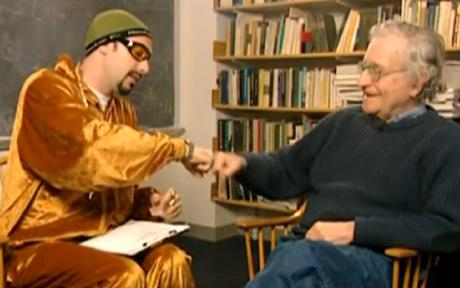
\includegraphics[scale=.5]{material/11chomksy}
	\caption{Geschafft!}
\end{figure}
	
\end{frame}

